\documentclass{beamer}
\usetheme{metropolis}           % Use metropolis theme
\usepackage{graphicx} % For including images
\usepackage{tikz}     % For positioning and layering
\usetikzlibrary{arrows.meta}
\usepackage{transparent}
\usepackage{url} % For handling URLs
\usepackage{tcolorbox} % For creating pretty boxes
\usetikzlibrary{backgrounds}
\usepackage{caption}
\usepackage{subcaption}
\usepackage{tikz}
\usepackage{algorithm}
\usepackage{algpseudocode}
\usepackage{float}
\usetikzlibrary{graphs, positioning}

% Hyperlinks
\hypersetup{
    colorlinks=true,
    linkcolor=secondary,
    urlcolor=black,
    citecolor=secondary
}

% Colors
\definecolor{primary}{HTML}{23373B}
\definecolor{secondary}{HTML}{38774D}
\definecolor{accent}{HTML}{E74C3C}
\definecolor{bg}{HTML}{ECF0F1}

% Define a custom tcolorbox style for definitions
\tcbset{
    colframe=blue!75!black,
    colback=bg,
    coltitle=primary,
    boxrule=1pt,
    fonttitle=\bfseries, % Bold title
    coltitle=white, % Title color
    boxrule=0.75mm, % Border thickness
    arc=2.5mm, % Rounded corners
    left=2mm, % Left padding
    right=2mm, % Right padding
    top=1mm, % Top padding
    bottom=1mm % Bottom padding
}

% for the sources of images: very small footnotes
\newcommand{\sourcefootnote}[1]{\let\thefootnote\relax\footnote{{\tiny Source: \url{#1}}}}

\title{Temporal Graphs}
% \subtitle{Algorithmic Gems for Graphs, Probabilities and Processes}

\date{January 28, 2025}

\author{Daniel Cermann}

\institute{
	\hfill \begin{minipage}{0.3\textwidth}
		\begin{center}
			
\includegraphics[width=60px]{media/hpi_logo.png} \newline
			Hasso Plattner Institute 
		\end{center}
	\end{minipage}
}

\begin{document}

\begin{frame}[label=potsdam_map]
	\begin{center}
		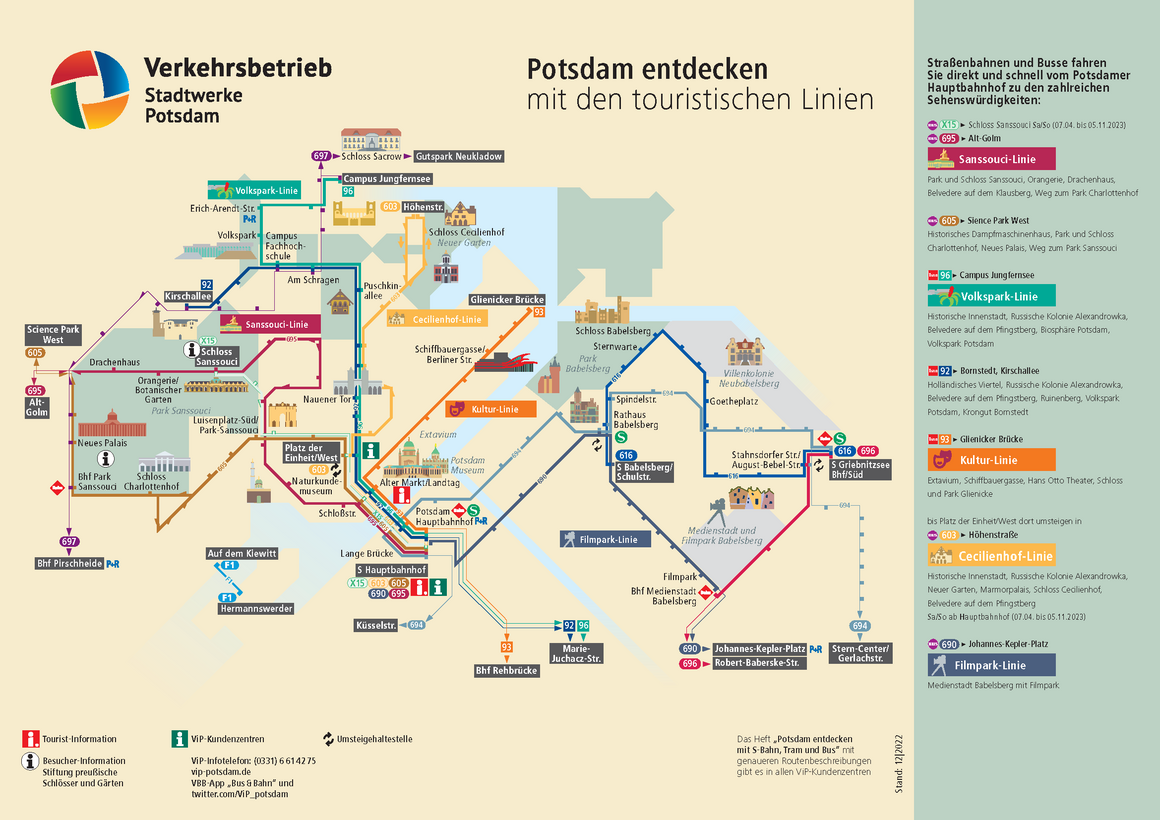
\includegraphics[width=0.95\textwidth]{media/potsdam_citynet.png}
	\end{center}
	\sourcefootnote{https://www.swp-potsdam.de/content/verkehr/bilder_6/liniennetz/touristischer_liniennetzplan_screenshot_1280_960.jpg}
\end{frame}

\maketitle

\section{Motivation}

\begin{frame}{Clip: School day}
	\url{https://youtu.be/BSNJSUkc5-Q?t=996}
\end{frame}

\begin{frame}{Google Maps}
	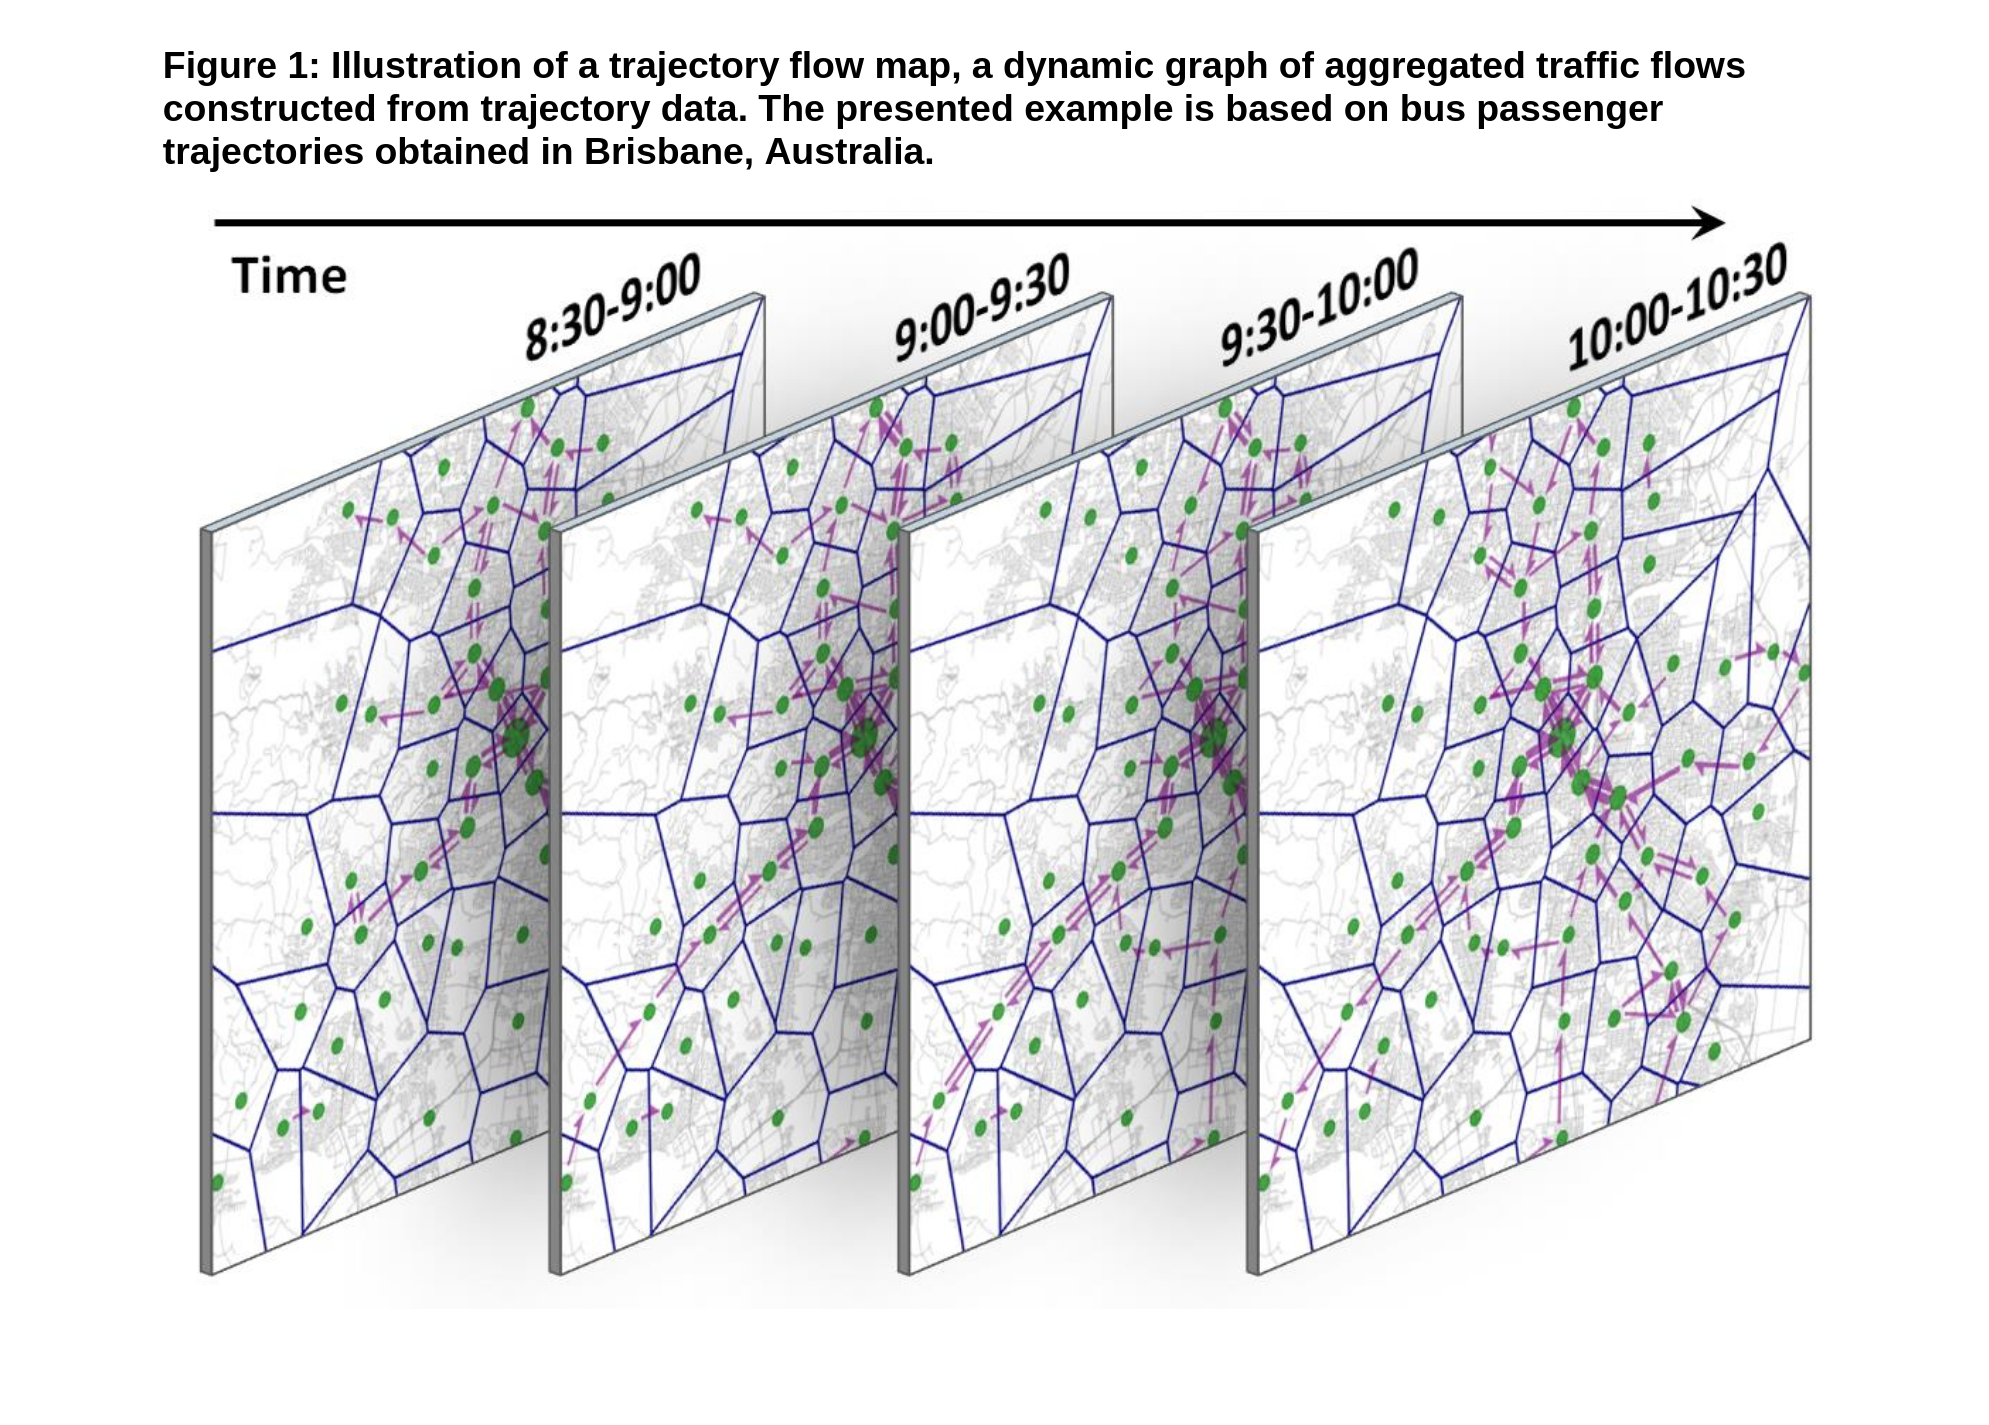
\includegraphics[width=0.9\linewidth]{media/temporal_traffic_data.png} 
	\sourcefootnote{https://australasiantransportresearchforum.org.au/wp-content/uploads/2022/03/ATRF2016_paper_166.pdf}
\end{frame}

\begin{frame}{Distributed systems}
	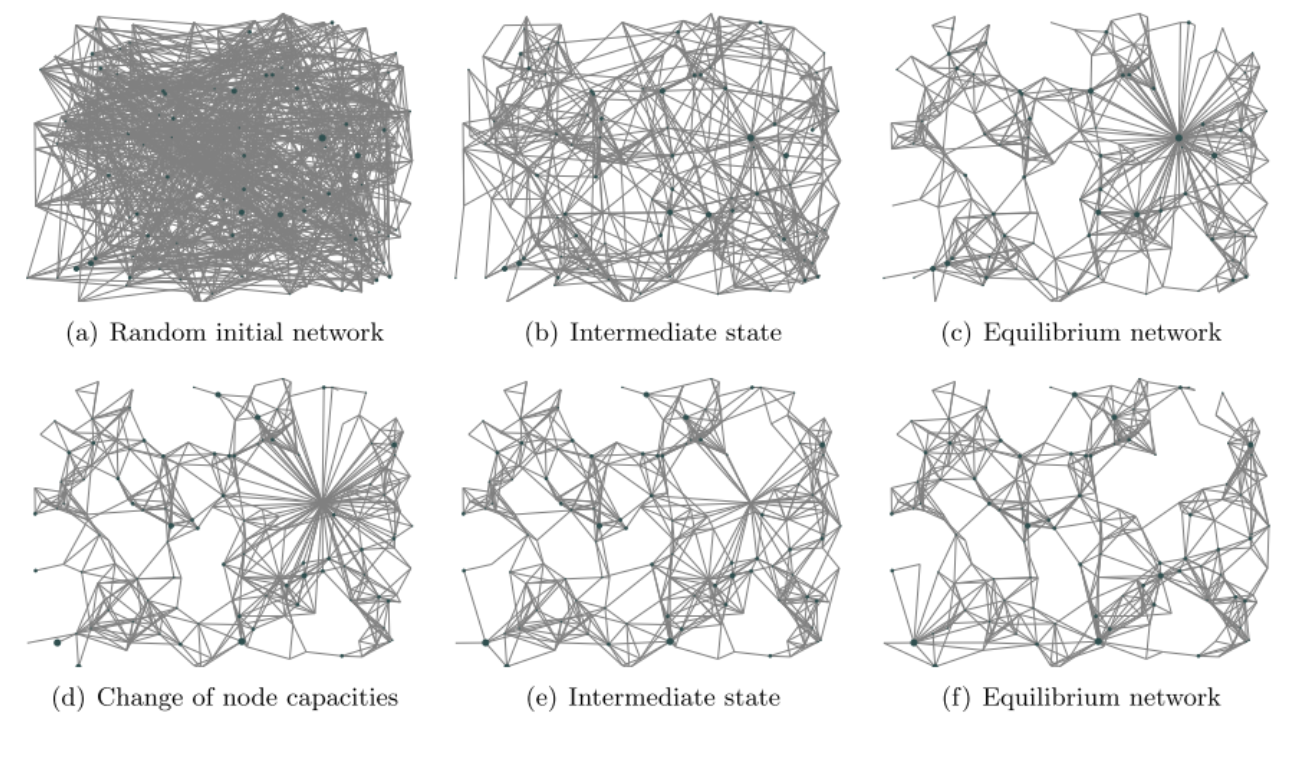
\includegraphics[width=\linewidth]{media/massive_distributed_system.png}
	\sourcefootnote{https://www.sg.ethz.ch/publications/2012/scholtes2012organic-design-of/}
\end{frame}

\begin{frame}{Temporal graphs for physical/chemical models}
	\begin{center}
	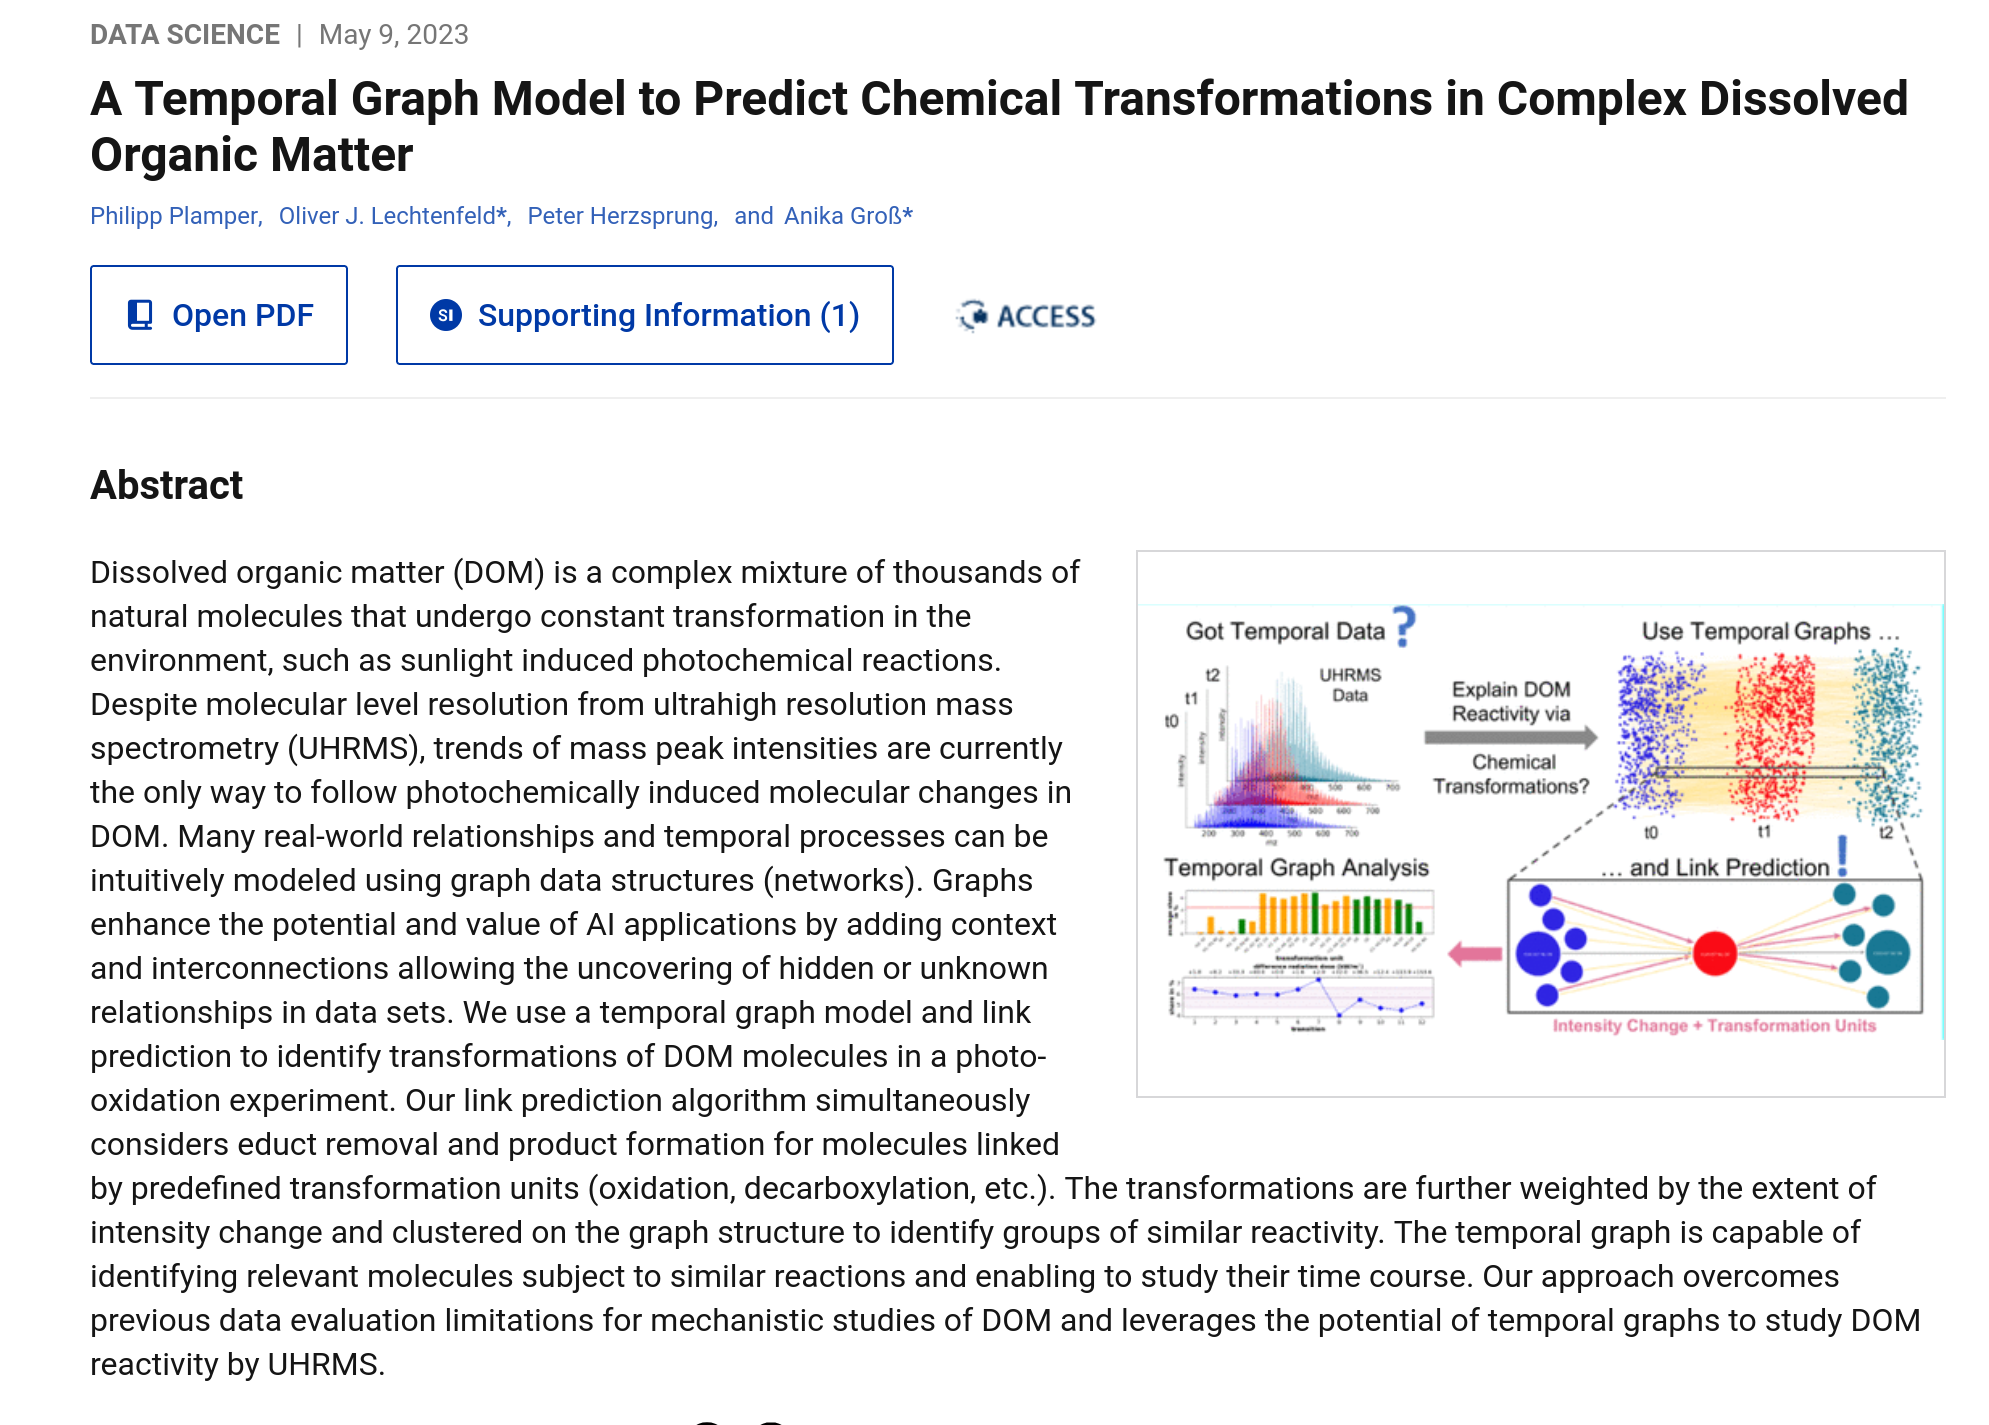
\includegraphics[width=0.8\linewidth]{media/organic_chemistry.png}
	\end{center}
	\sourcefootnote{https://pubs.acs.org/doi/full/10.1021/acs.est.3c00351}
\end{frame}

\begin{frame}{Dissemination processes}
  \centering
  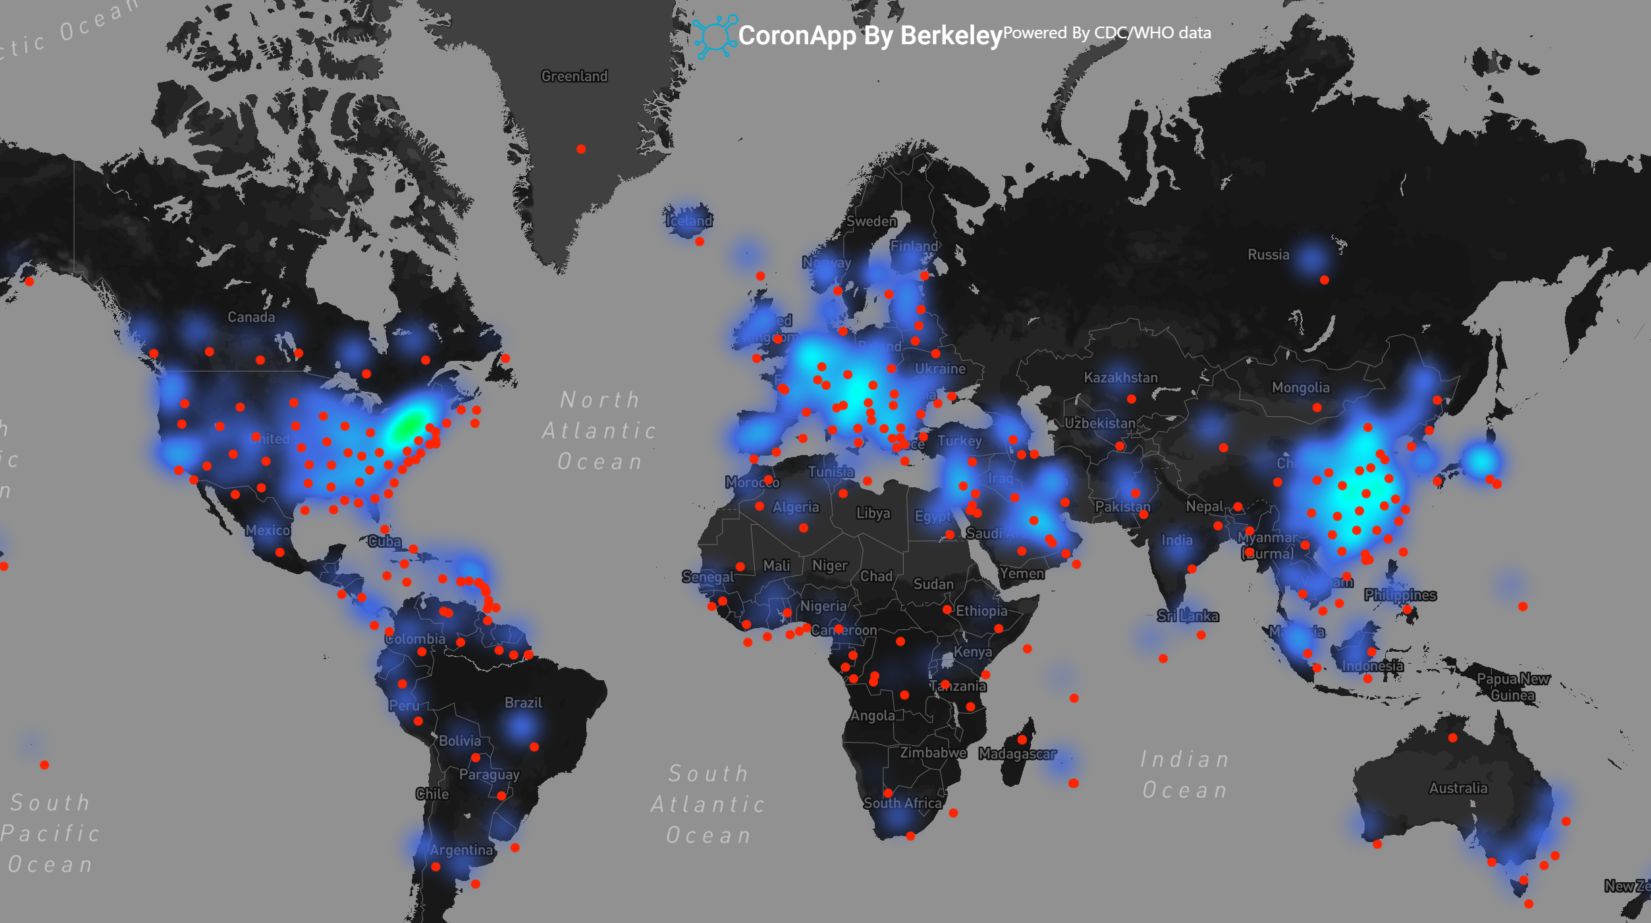
\includegraphics[width=\linewidth]{media/corona.png}
  \sourcefootnote{https://engineering.berkeley.edu/wp-content/uploads/2020/03/CoronApp.png}
\end{frame}

\section{How to model temporal graphs}

\begin{frame}{How to represent time in graphs?}
  \large 
  \italic{Brainstorm with your neighbor how time can be represented in graphs. Don't think of notation for now, just some visual ways to represent the additional dimension.}
  \tiny \hfill $\approx$ 2 min \\[3ex]
  \centering
  \begin{minipage}{0.6\textwidth}
  \begin{center}
    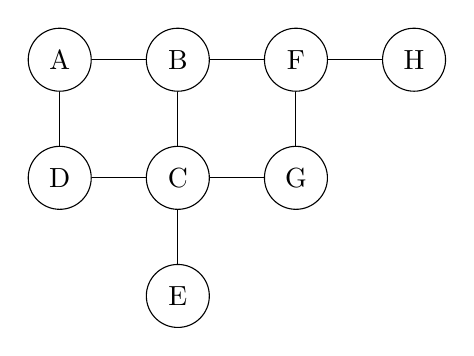
\begin{tikzpicture}[node distance=1.5cm, every node/.style={draw, circle, minimum size=0.8cm}]
        % Nodes
        \node (A) {A}; % High-risk node
        \node (B) [right of=A] {B};
        \node (C) [below of=B] {C}; % High-risk node
        \node (D) [below of=A] {D};
        \node (E) [below of=C] {E};
        \node (F) [right of=B] {F};
        \node (G) [below of=F] {G};
        \node (H) [right of=F] {H};

        % Edges
        \path (A) edge (B);
        \path (A) edge (D);
        \path (B) edge (C);
        \path (B) edge (F);
        \path (C) edge (D);
        \path (C) edge (E);
        \path (C) edge (G);
        \path (F) edge (G);
        \path (F) edge (H);
   \end{tikzpicture}
  \end{center}
  \end{minipage}
  \begin{minipage}{0.1\textwidth}
    \large +
  \end{minipage}
  \begin{minipage}{0.2\textwidth}
    \large ?
  \end{minipage}
\end{frame}


\begin{frame}{How to represent time in graphs?}
		\centering
		\begin{figure}
				\begin{subfigure}{0.42\textwidth}
						\centering
						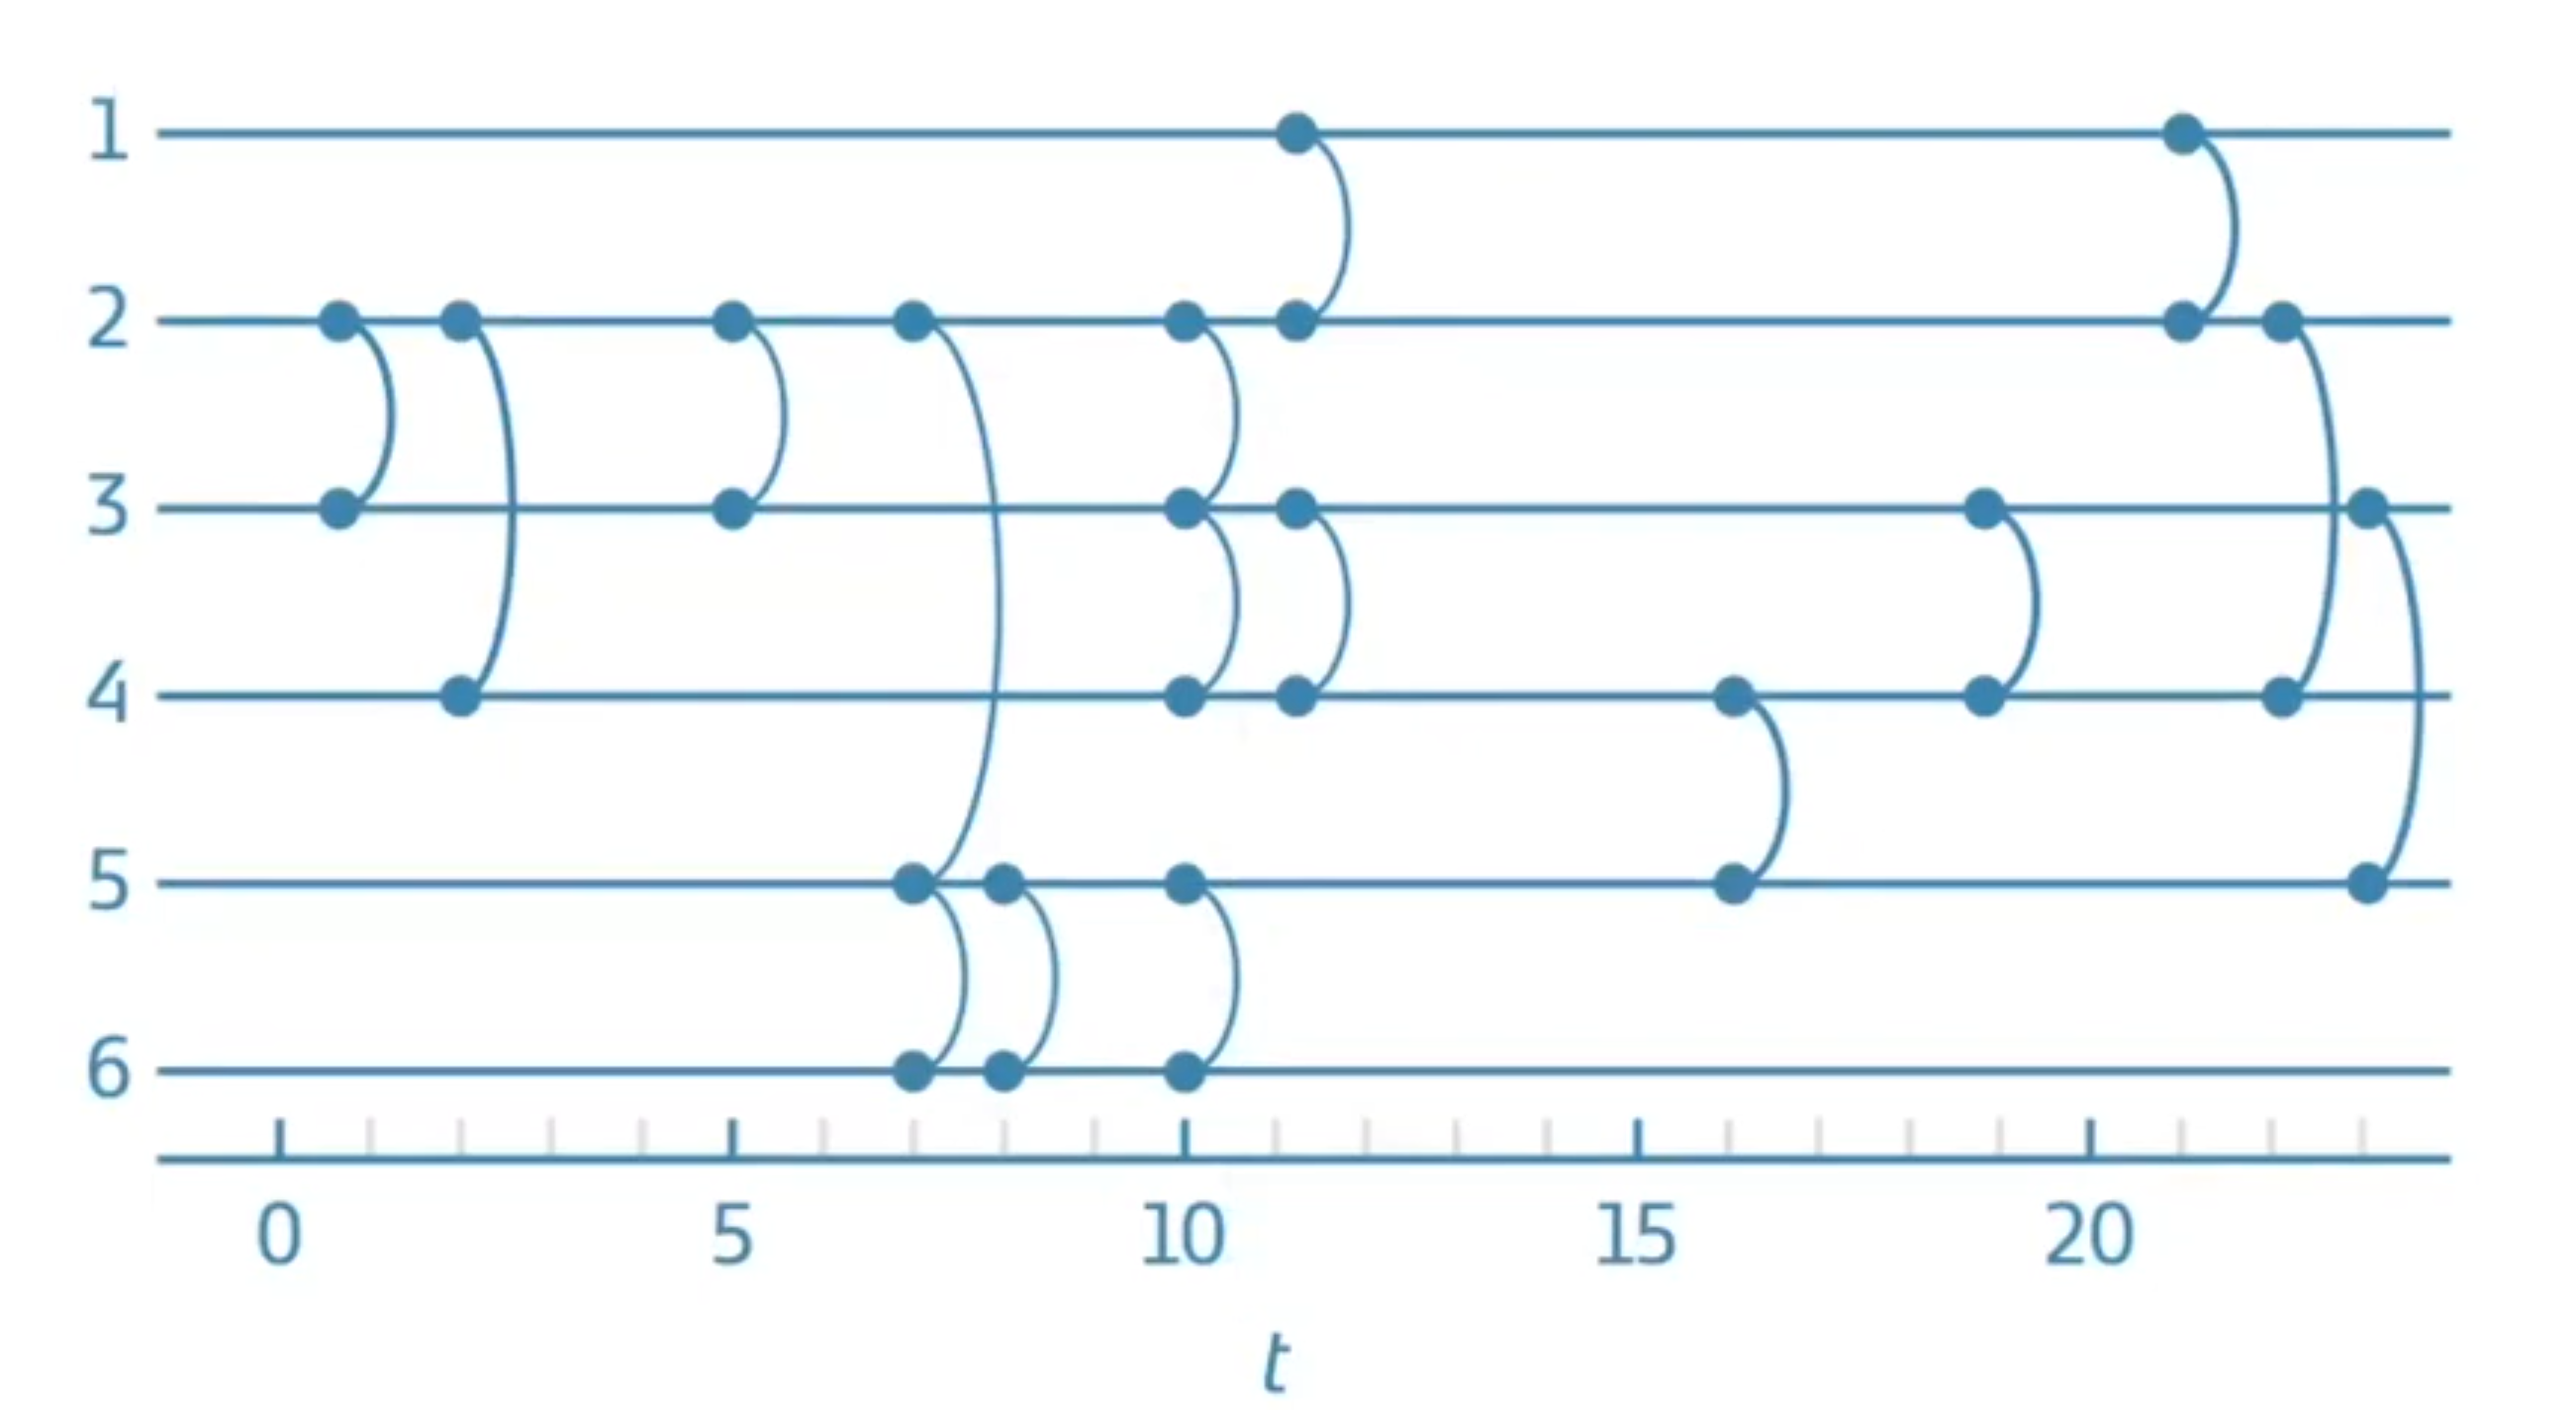
\includegraphics[width=\textwidth]{media/temporal_sense_1.png}
				\end{subfigure}
				\hfill
				\begin{subfigure}{0.42\textwidth}
						\centering
						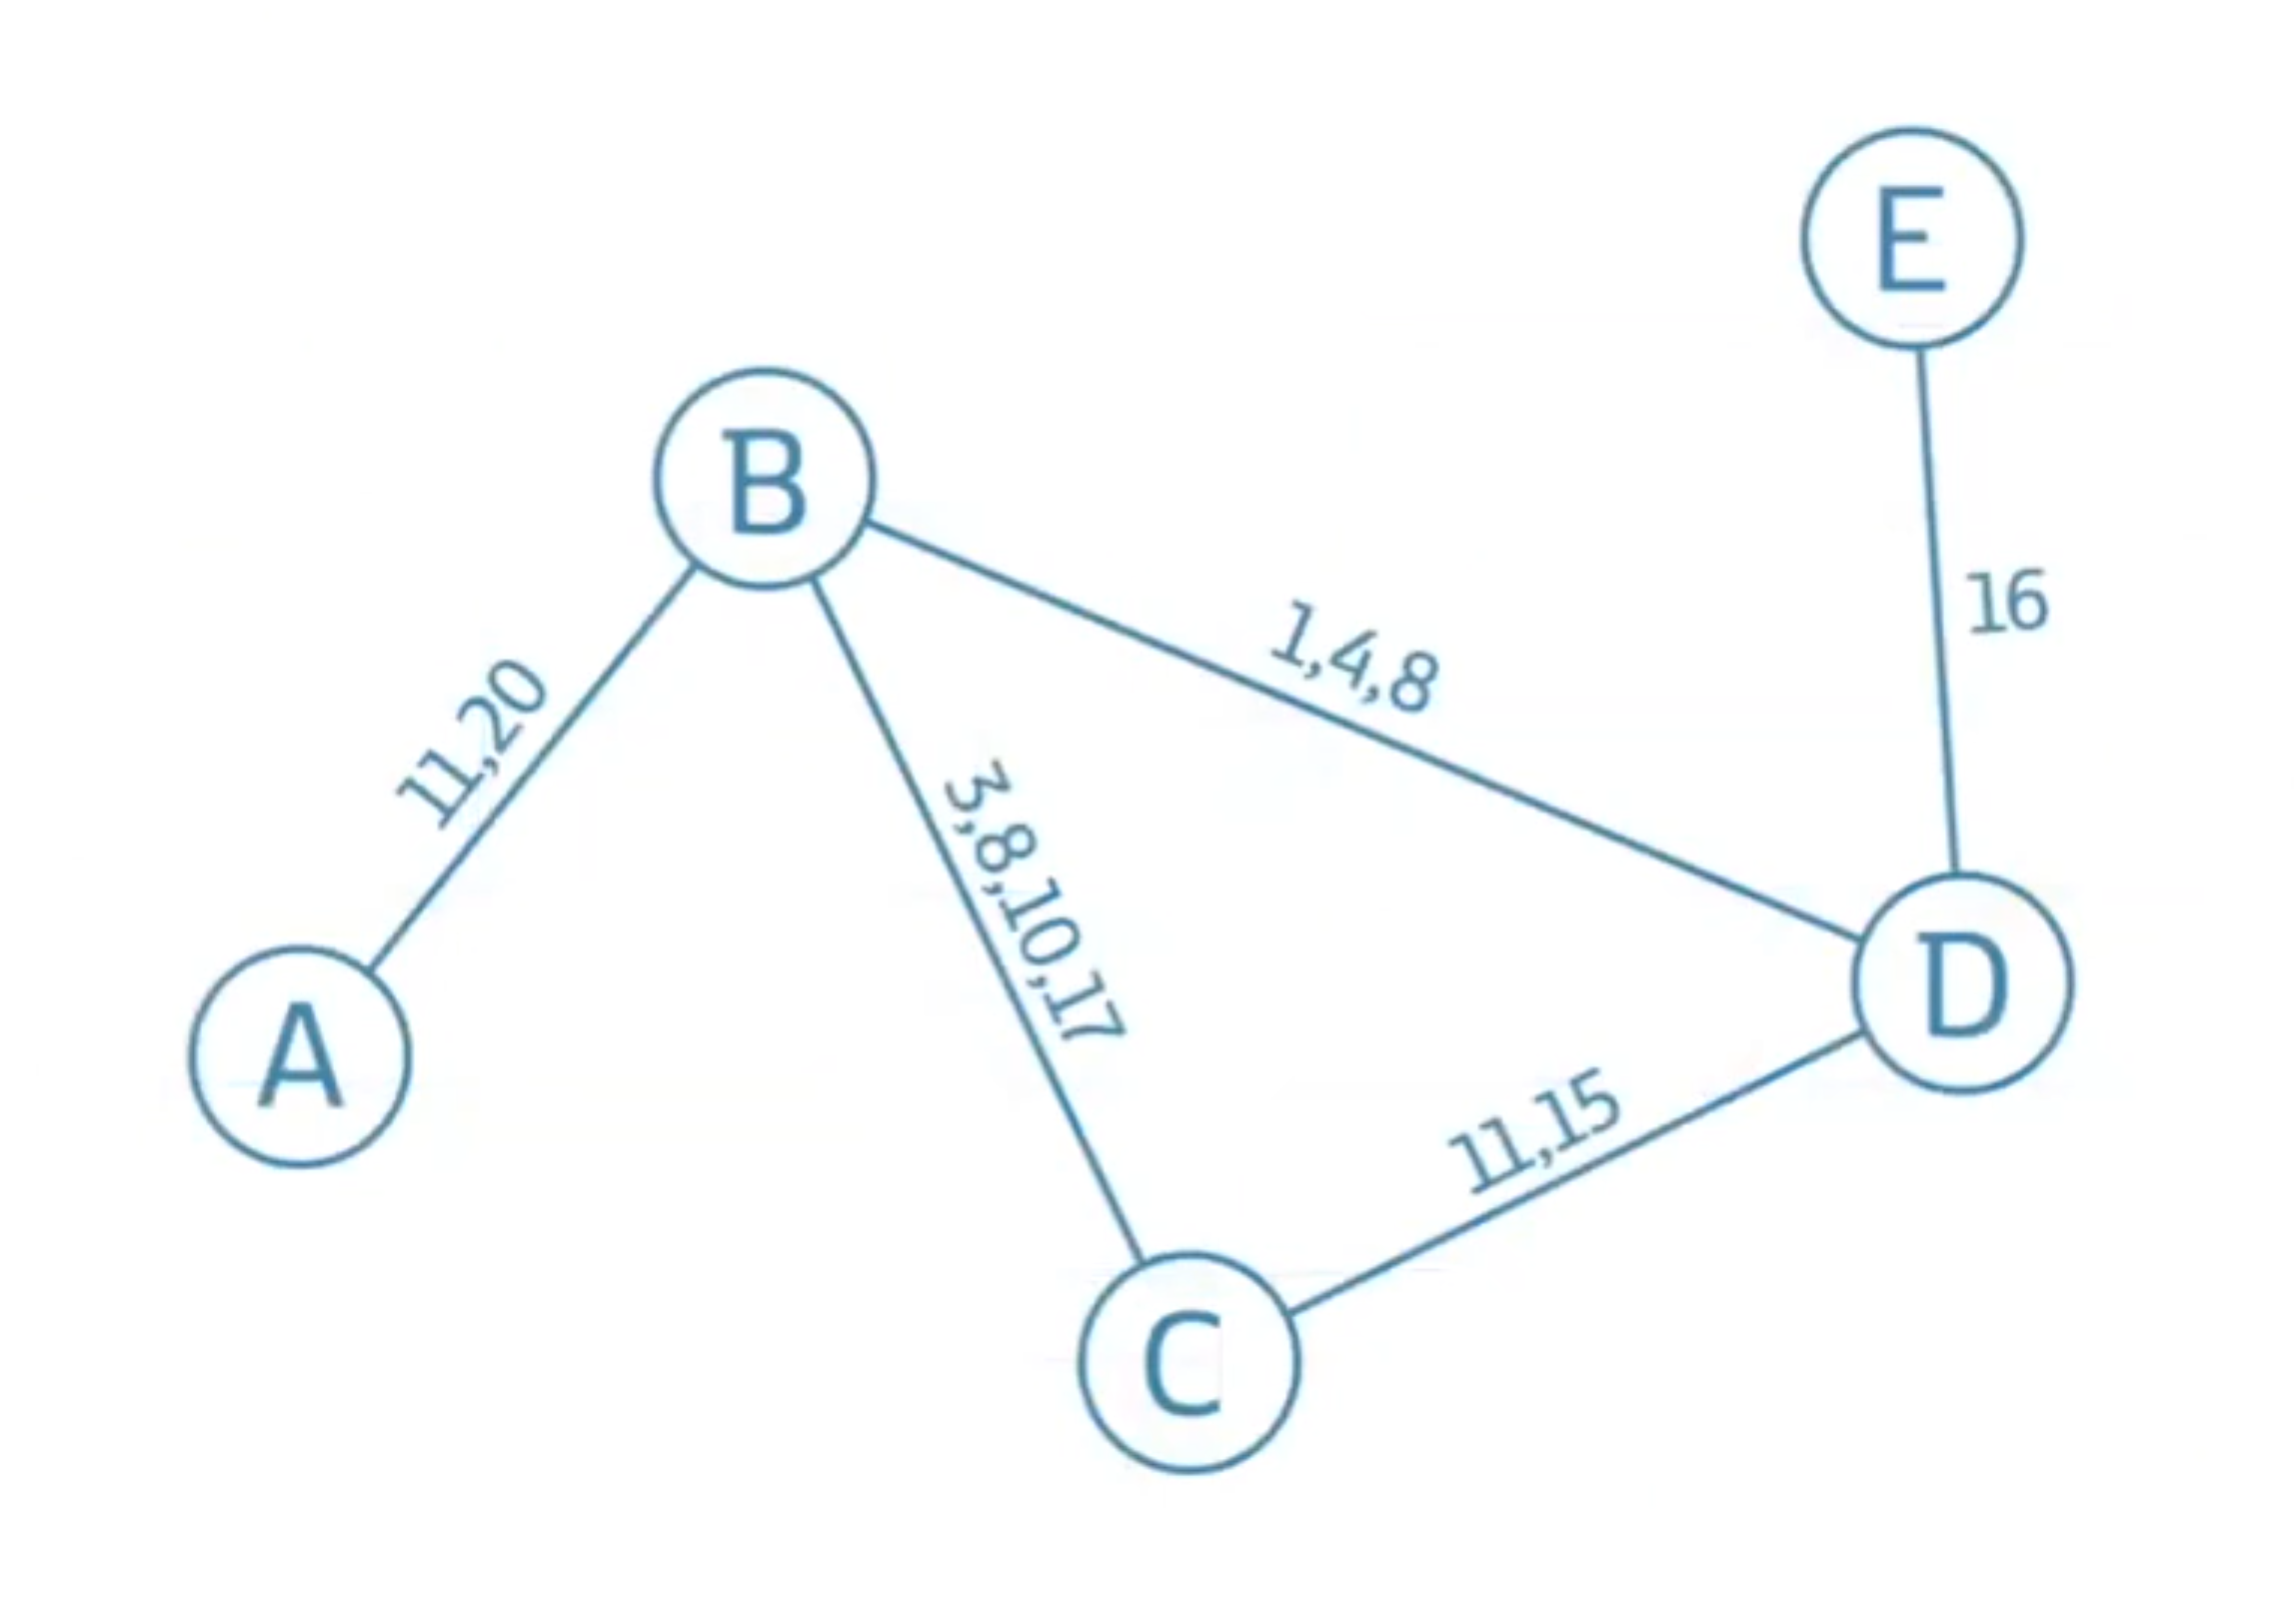
\includegraphics[width=\textwidth]{media/temporal_sense_2.png}
				\end{subfigure}

				\vspace{0.5cm} % Space between rows

				\begin{subfigure}{0.42\textwidth}
						\centering
						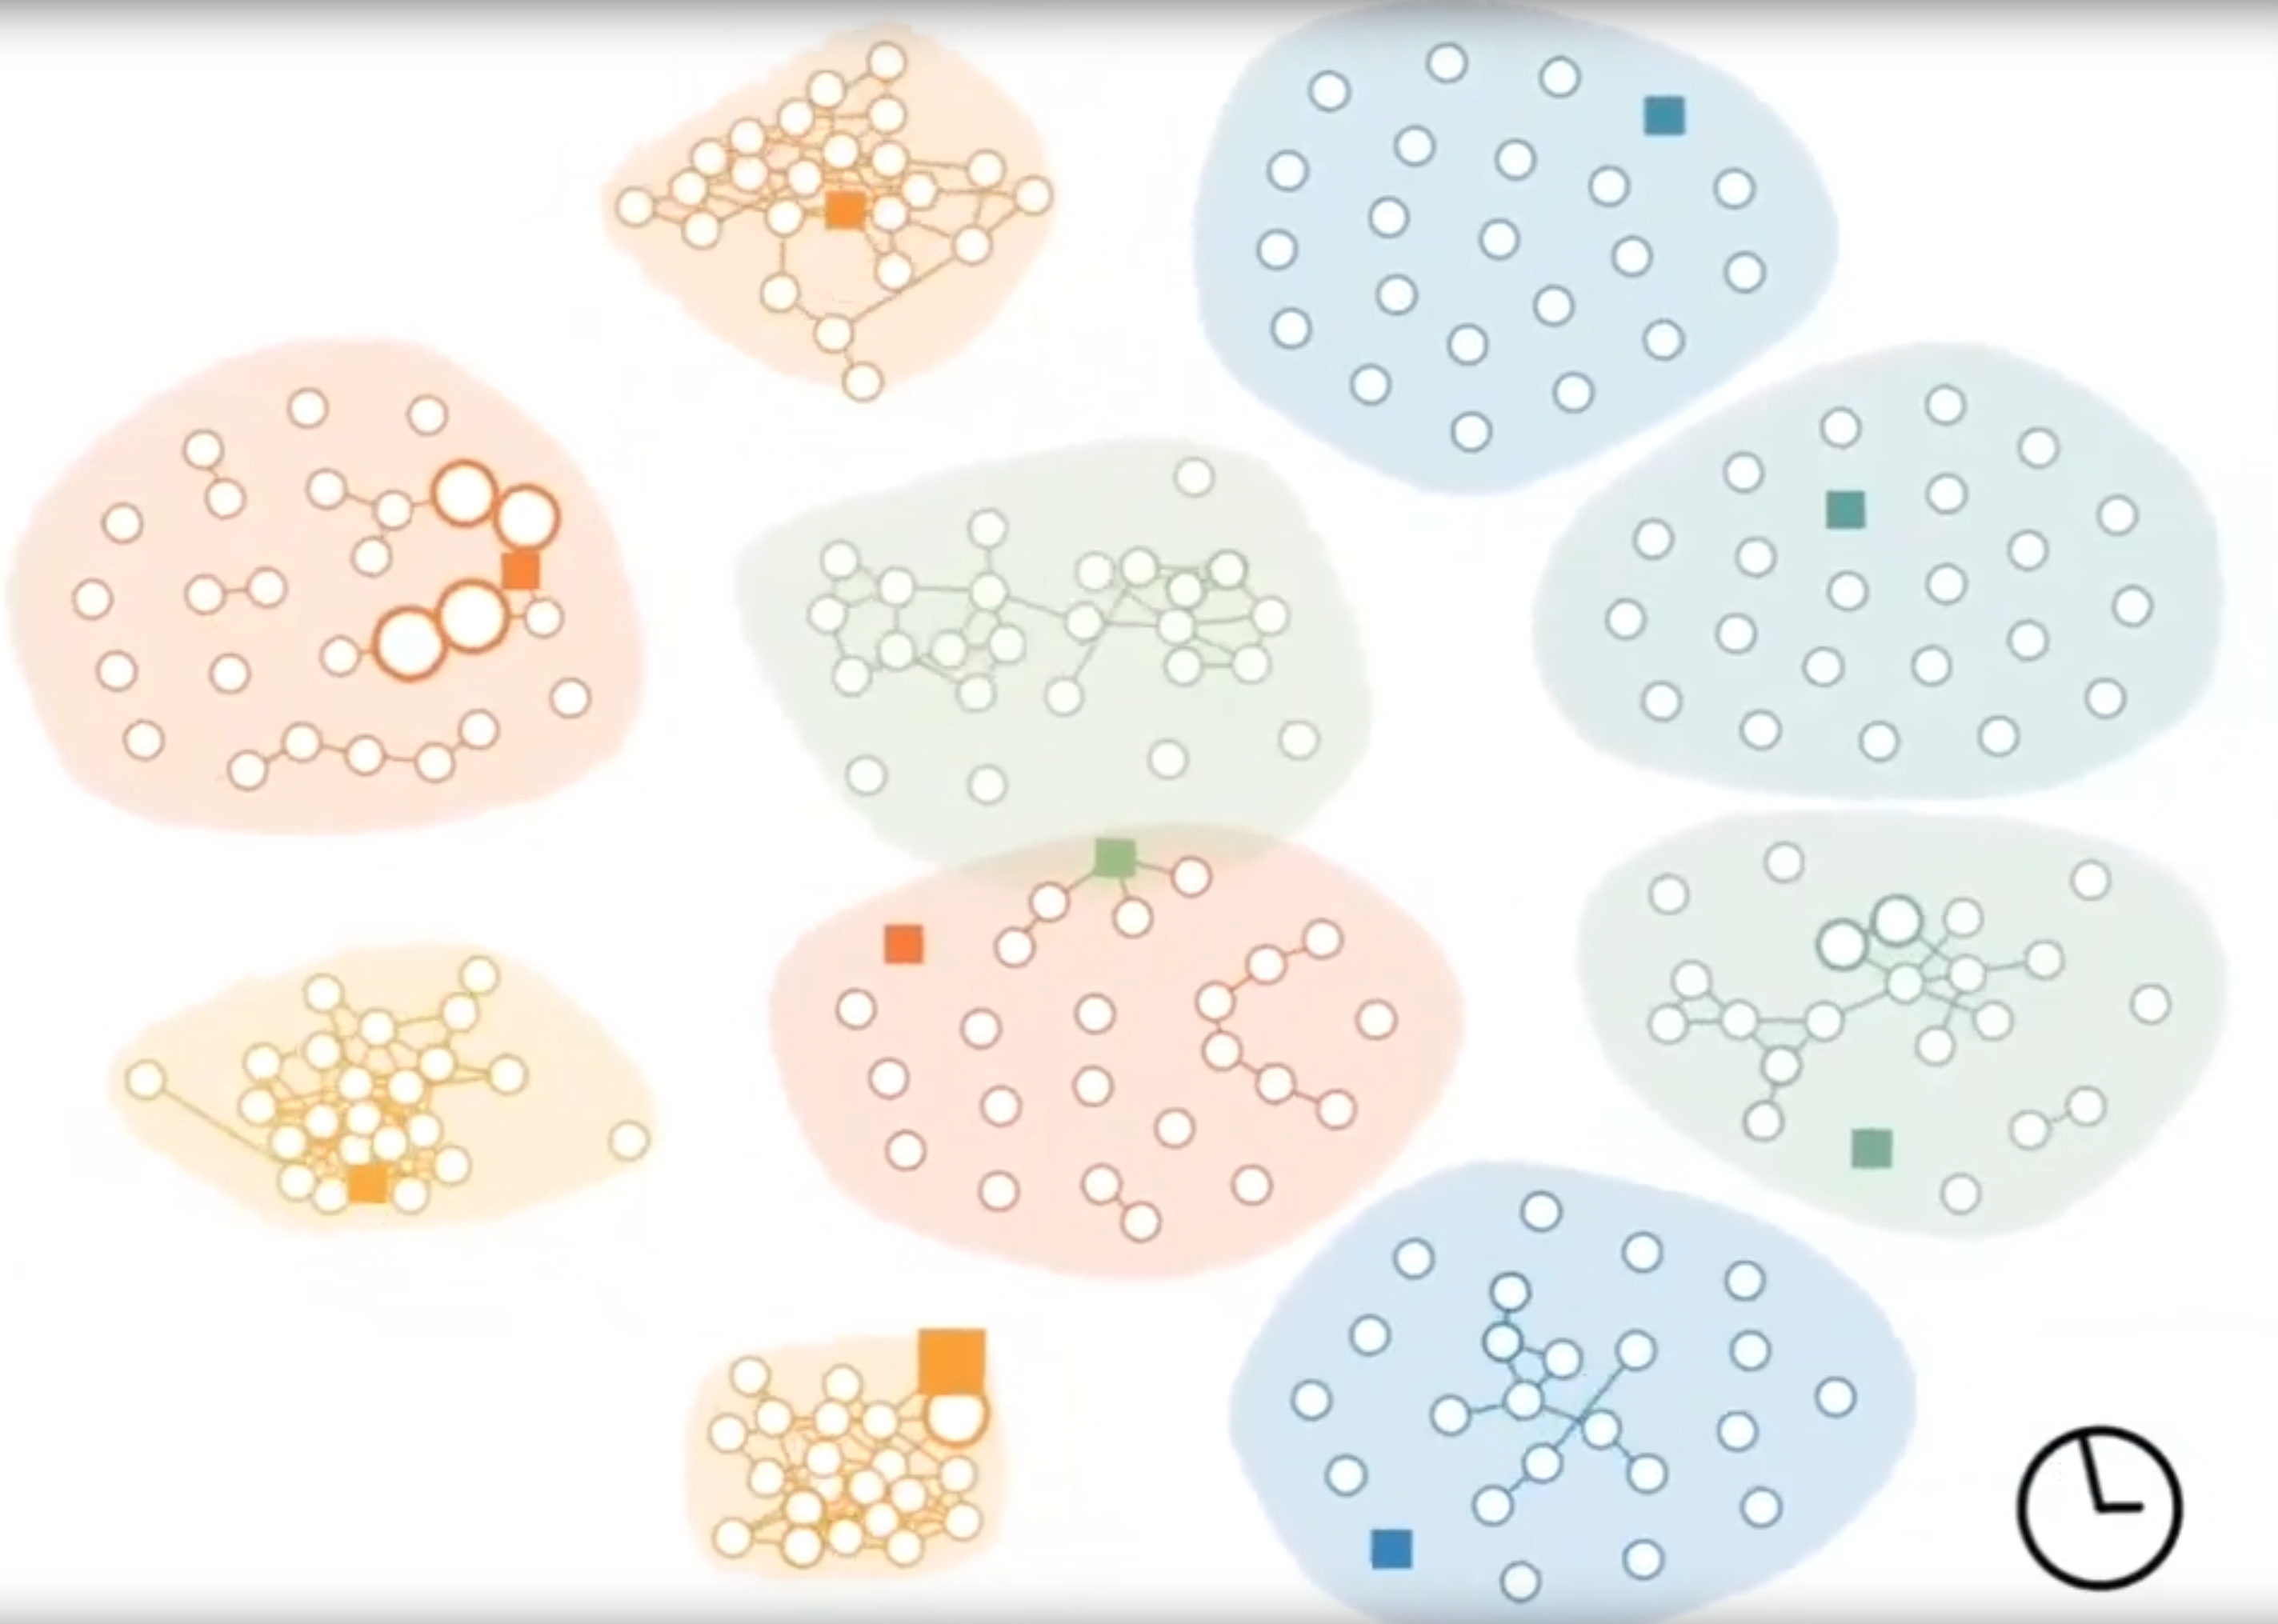
\includegraphics[width=\textwidth]{media/temporal_sense_3.png}
				\end{subfigure}
				\hfill
				\begin{subfigure}{0.42\textwidth}
						\centering
						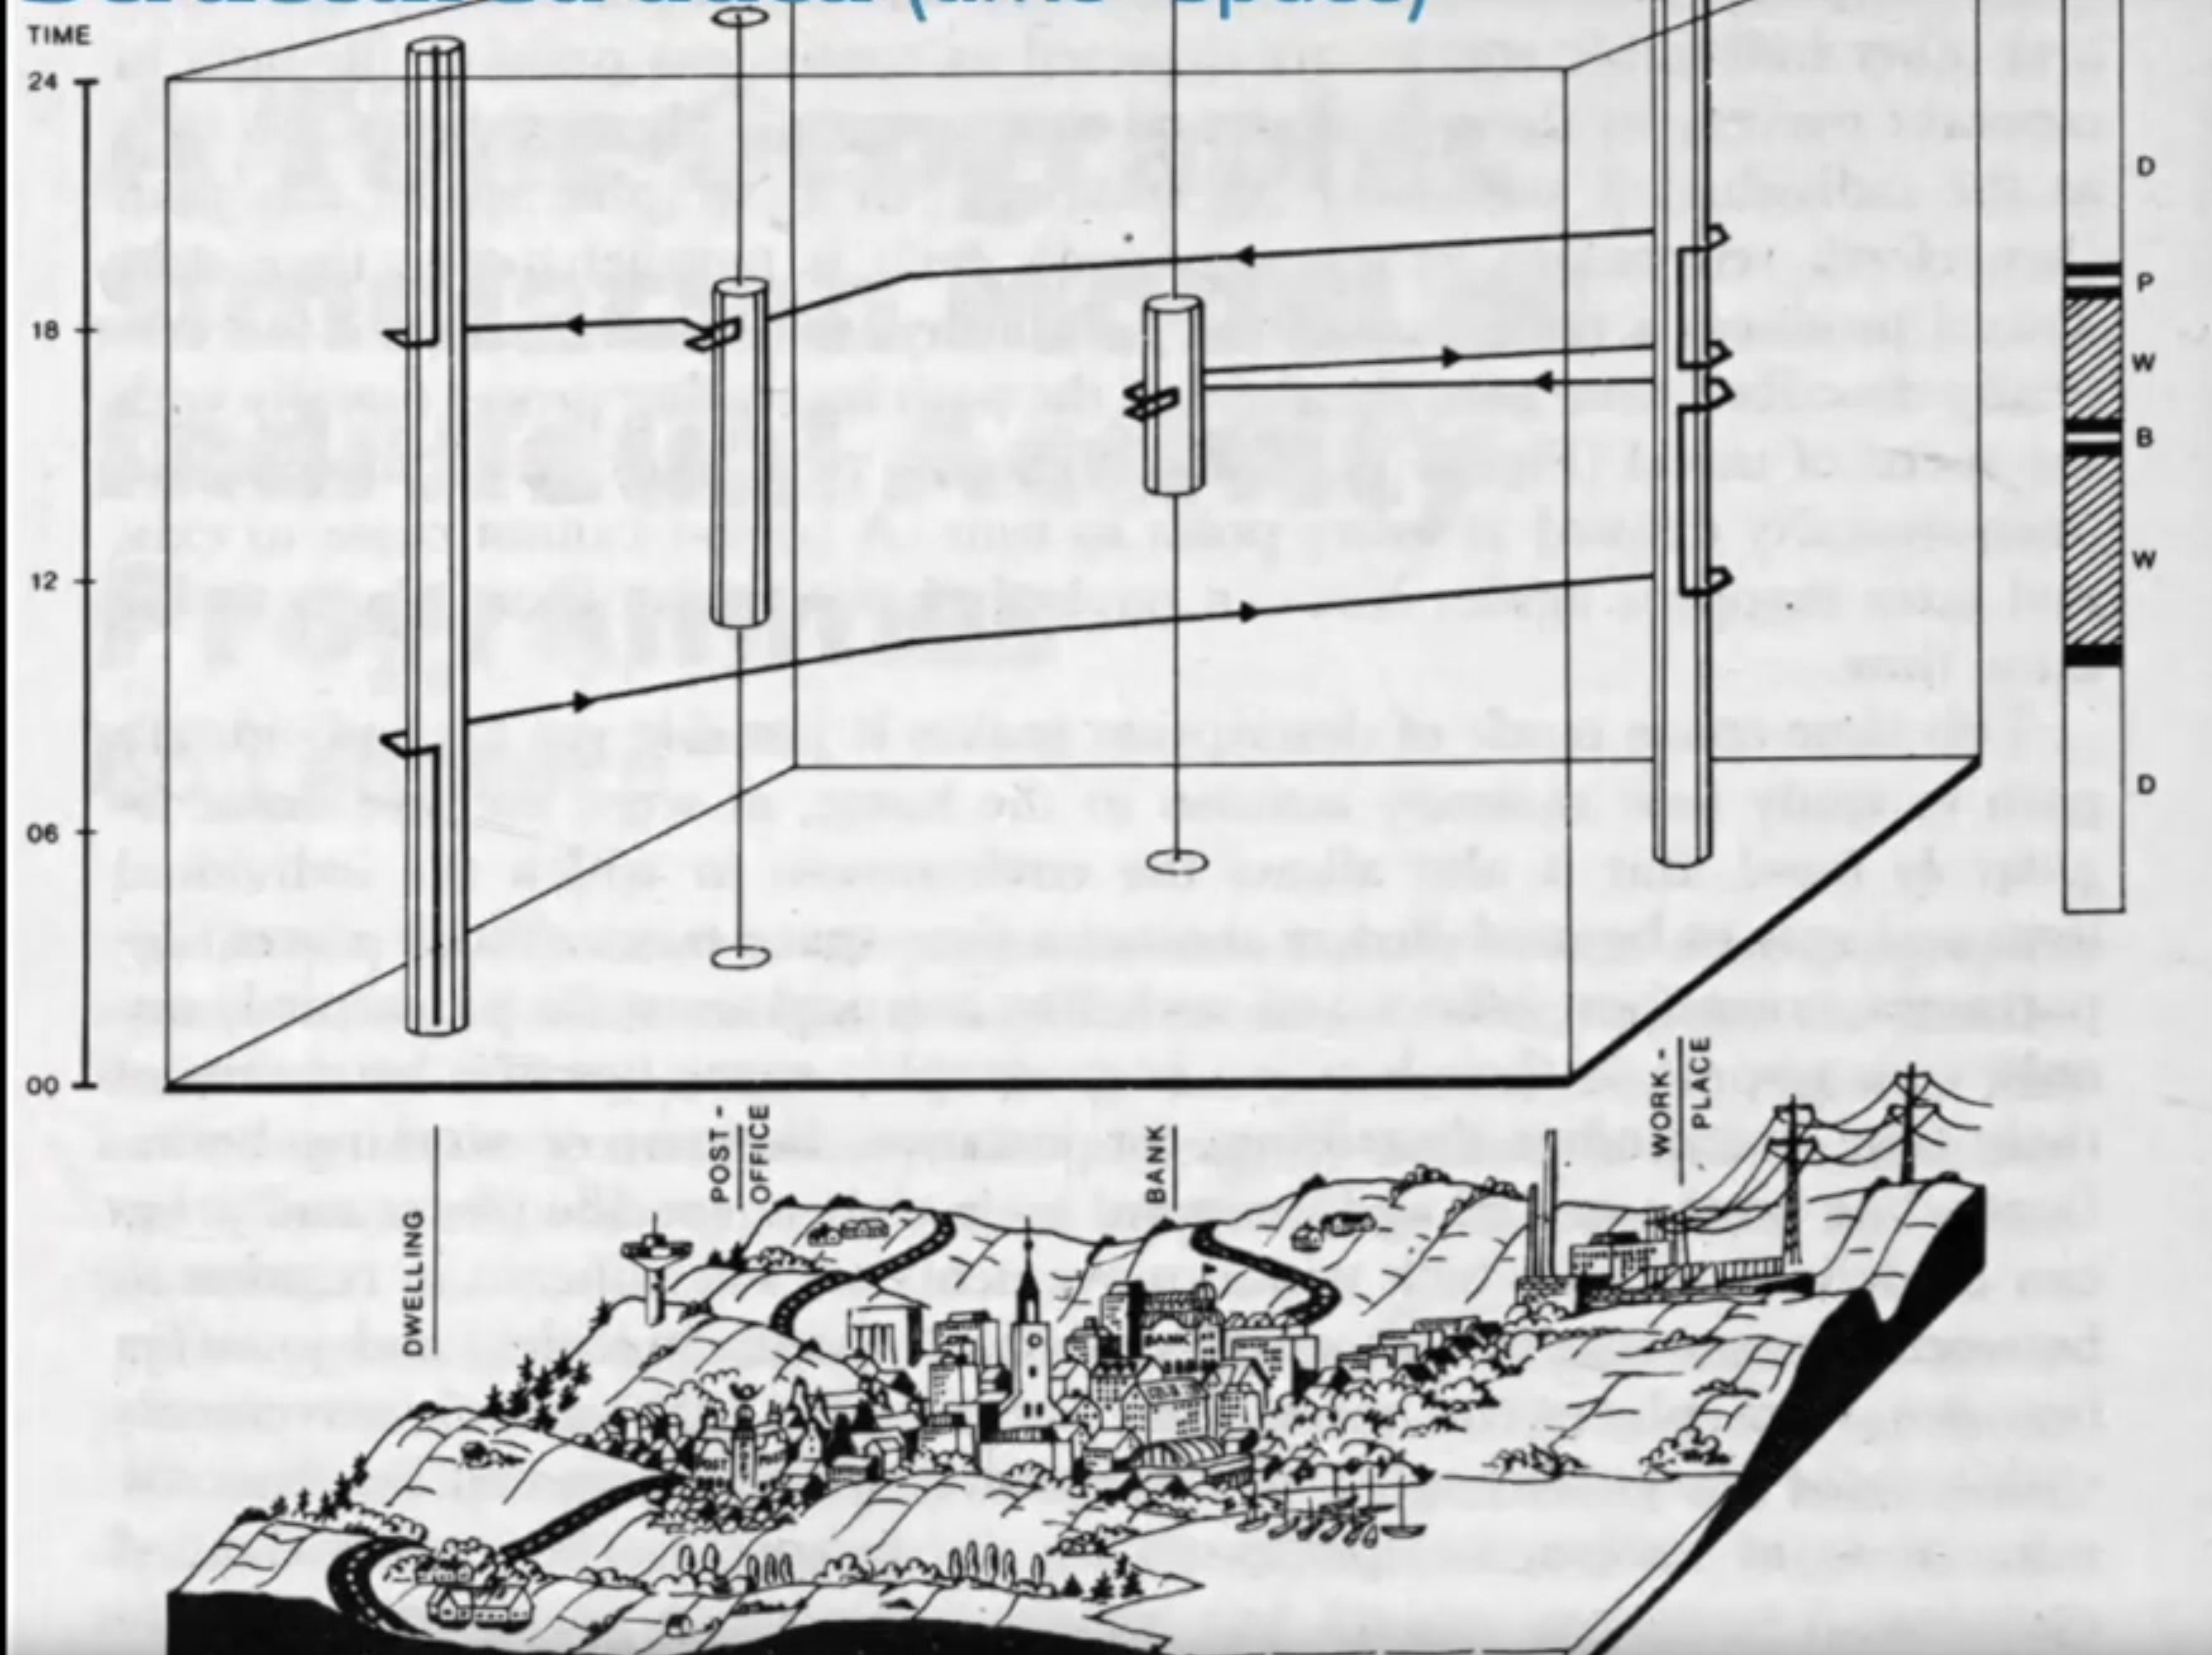
\includegraphics[width=\textwidth]{media/temporal_sense_4.png}
				\end{subfigure}
				\sourcefootnote{https://www.youtube.com/watch?v=BSNJSUkc5-Q}
		\end{figure}
\end{frame}

\begin{frame}{How to model temporal graphs}
	\centering
	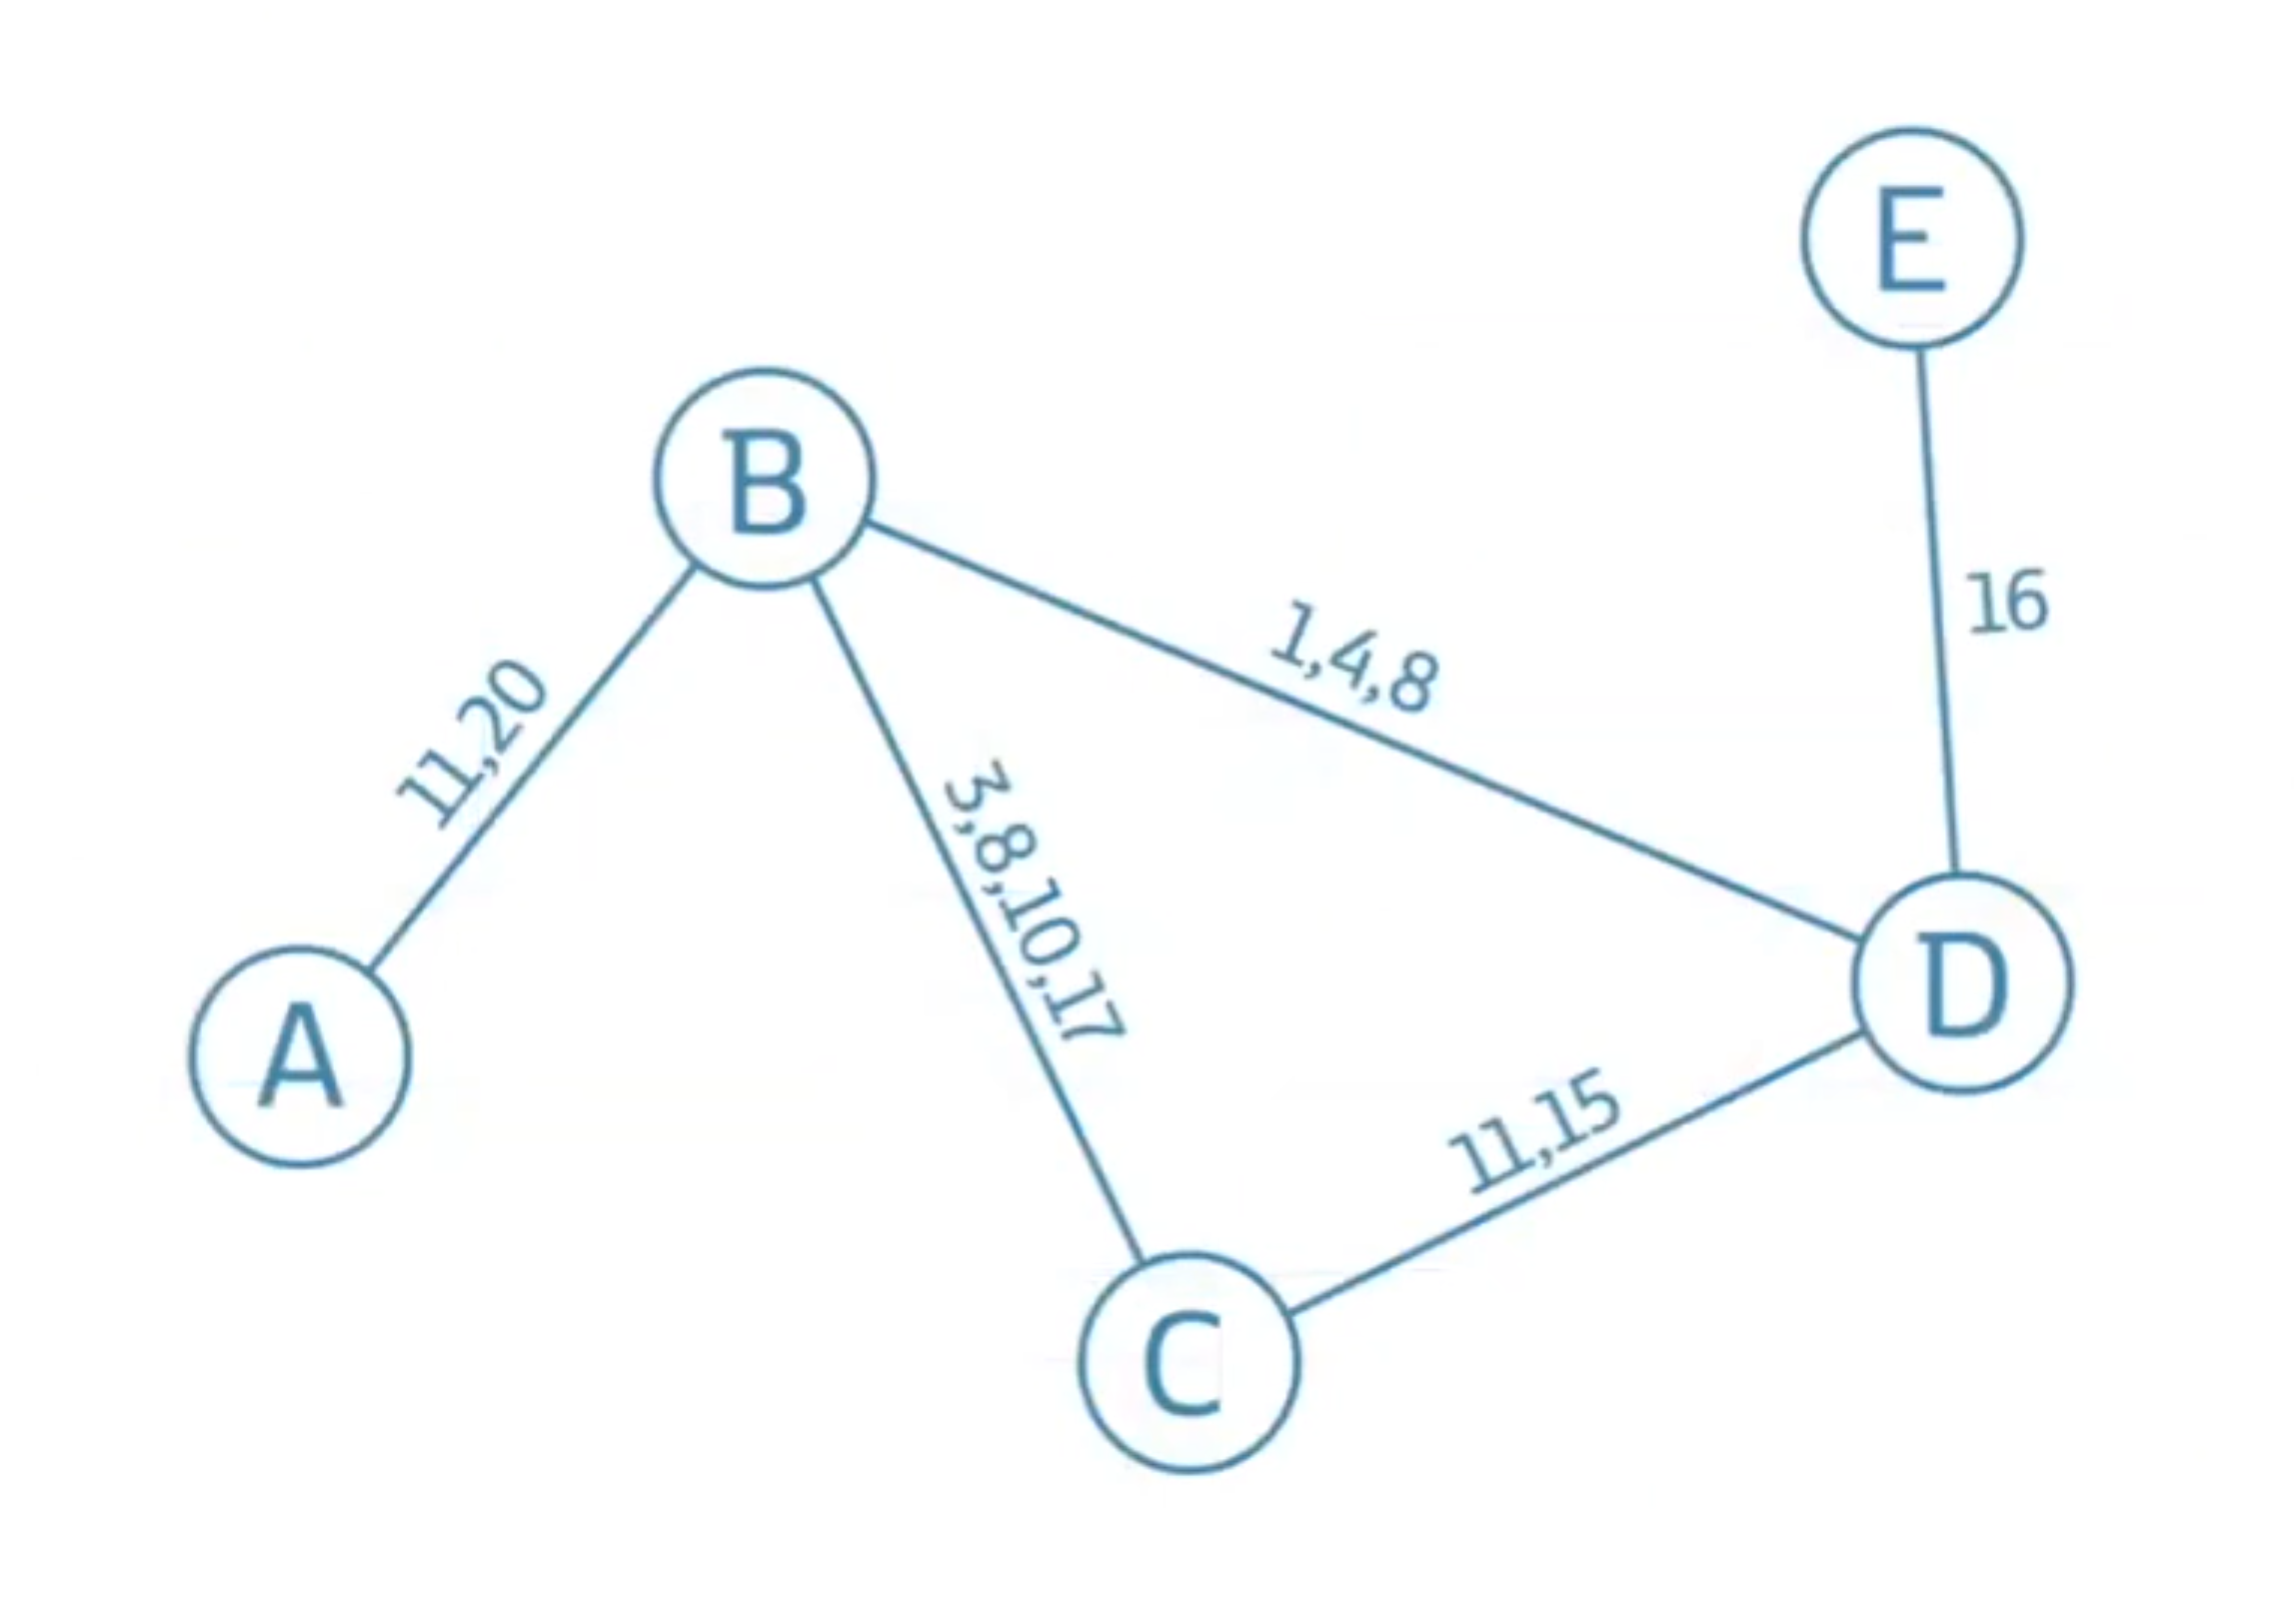
\includegraphics[width=0.9\linewidth]{media/temporal_sense_2.png}
	\sourcefootnote{https://www.youtube.com/watch?v=BSNJSUkc5-Q}
\end{frame}


\begin{frame}{Definition labeled and temporal graphs}
	\visible<1->{
		\begin{tcolorbox}[title=Definition]
			A \textbf{labeled graph} \cite[page 94]{GHOSH201888} is a triple \( G = (V, E, \lambda) \) where:
				\begin{itemize}
						\item \( (V, E) \) is a graph
						\item $ \lambda: V \cup E \rightarrow Z$ is a mapping of nodes and edges to a set of labels $Z$
					\end{itemize}
		\end{tcolorbox}
		}

	\visible<2->{
	 \begin{tcolorbox}[title=Definition]
			A \textbf{temporal graph} \cite[page 243]{Michail2015} is is triple \( G = (V, E, \lambda) \) where:
			\begin{itemize}
						\item \( V, E \) is a graph
						\item $ \lambda: E \rightarrow 2^{\mathbb{N}}$ is a mapping of edges to a set natural numbers (time steps when this edge is active)
					\end{itemize}
		\end{tcolorbox}
	}
\end{frame}

\begin{frame}{Relationship labeled and temporal graphs}
  \begin{minipage}{0.45\textwidth}
    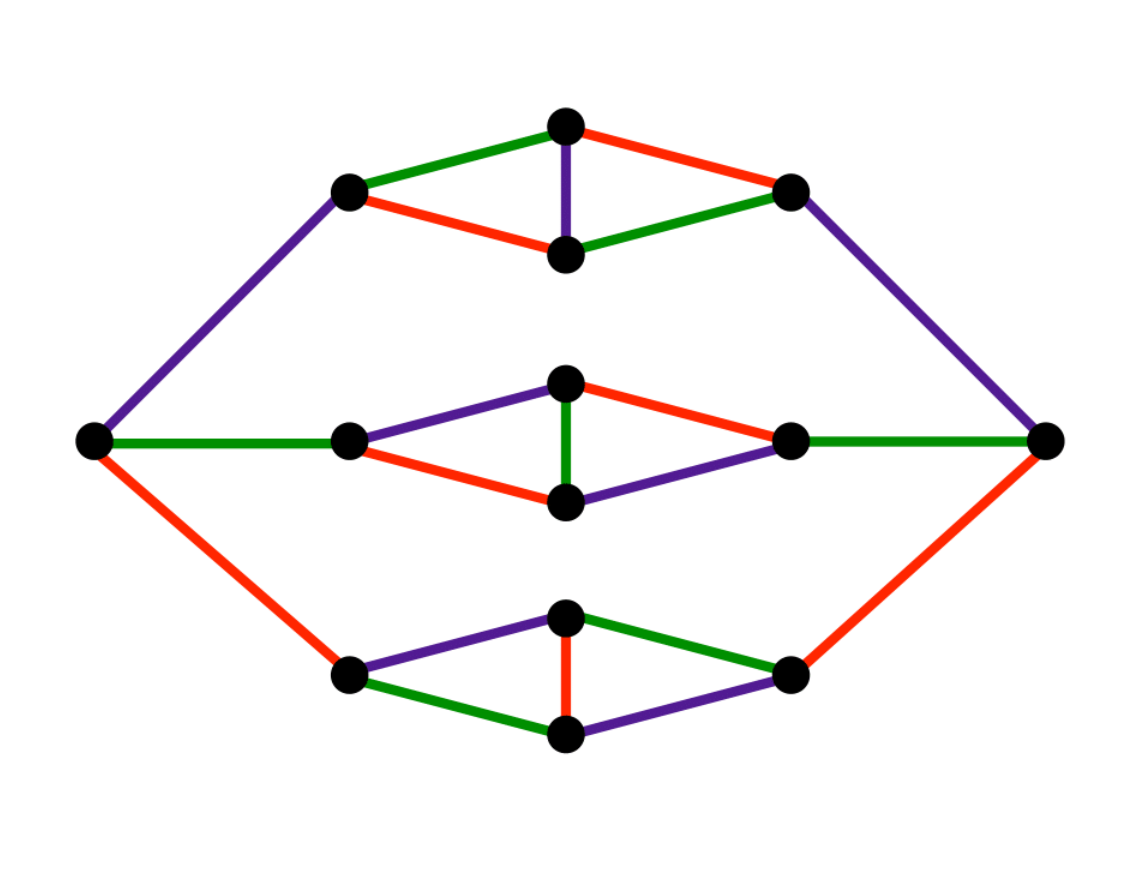
\includegraphics[width=\linewidth]{media/proper_edge_coloring.png}
    \sourcefootnote{https://www.algorist.com/images/figures/edge-coloring-R.png}
  \end{minipage}
  \hfill $\leftrightarrow$ \hfill
  \begin{minipage}{0.45\textwidth}
  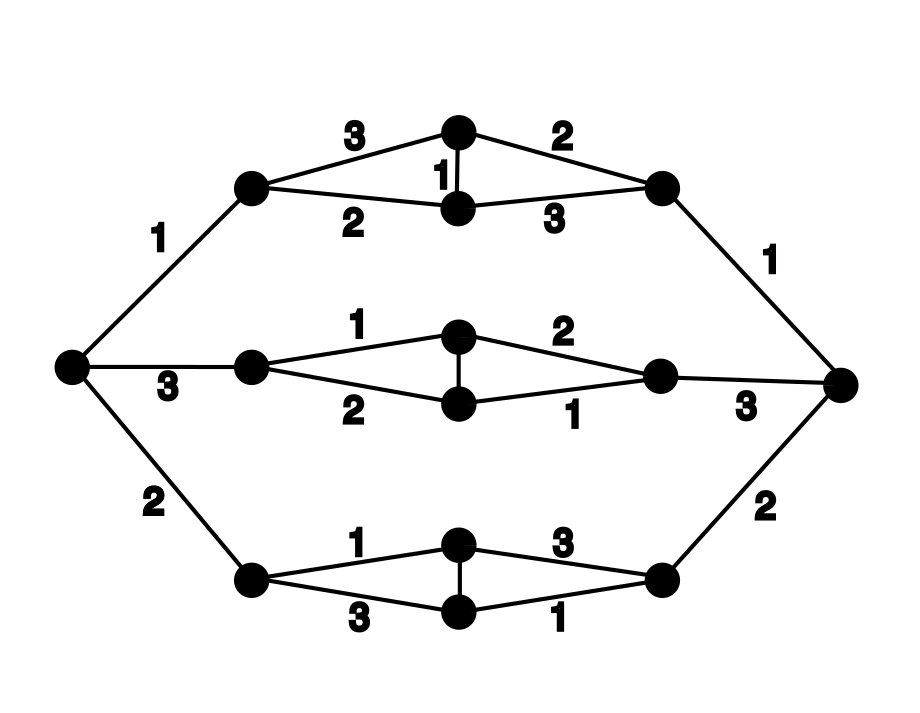
\includegraphics[width=\linewidth]{media/edge_coloring_to_temporal_graph.png}
  \sourcefootnote{me :)}
  \end{minipage}
\end{frame}

\begin{frame}{Exercise notation}
  \large
  \italic{Given the following temporal graph definition $D = (V, E, \lambda)$ draw the visual representation of the temporal graph on the template in the handout!} \hfill \tiny $\approx$ 2 min \\
  \normal
  $$ V = \{ C, H, B, P, M, G, W \} $$
  $$ E = \{ (C, H), (H, B), (B, G), (G, W), (W, P), (H, P), (B, M), (M, G) $$
  $$  \qquad (H, C), (B, H), (G, H), (W, G), (P, W), (P, H), (M, B), (G, M) \} $$
  \hfill \begin{minipage}{0.6\textwidth}
  $ \lambda = \{ \newline
    \hspace*{1cm}  (C, H) \mapsto \{ 1, 4 \}, \newline
    \hspace*{1cm}  (H, C) \mapsto \{ 4, 7 \}, \newline
    \hspace*{1cm}  (H, B) \mapsto \{ 2, 5 \}, \newline
    \hspace*{1cm}  (B, H) \mapsto \{ 3, 6 \}, \newline
    \hspace*{1cm}  (B, G) \mapsto \{ 3, 6 \}, \newline
    \hspace*{1cm}  (G, B) \mapsto \{ 2, 5 \}, \newline
    \hspace*{1cm}  (G, W) \mapsto \{ 4, 7 \}, \newline
    \hspace*{1cm}  (W, G) \mapsto \{ 1, 4 \}, \newline
    \hspace*{1cm}  (H, M) \mapsto \{ 2, 5 \}, \newline
    \hspace*{1cm}  (M, H) \mapsto \{ 3, 6 \}, \newline
    \hspace*{1cm}  (M, W) \mapsto \{ 3, 6 \} \newline
    \hspace*{1cm}  (W, M) \mapsto \{ 2, 5 \} \newline
    \hspace*{1cm}  (B, P) \mapsto \{ 1, 4, 7 \} \newline
    \hspace*{1cm}  (P, B) \mapsto \{ 2, 5, 8 \} \newline
    \hspace*{1cm}  (G, P) \mapsto \{ 2, 5, 8 \} \newline
    \hspace*{1cm}  (P, G) \mapsto \{ 1, 4, 7 \} \newline
        \} $ 
  \end{minipage} \hfill
\end{frame}

\begin{frame}[label=potsdam_city_graph]{Solution}
\begin{tikzpicture}[
    every node/.style={circle, draw, minimum size=0.3cm, font=\small},
    every edge/.style={draw, ->, font=\tiny},
    labelstyle/.style={draw=none, font=\tiny, midway, maximum size=0.3cm, inner sep=0.1pt},
    >=stealth
]

% Define vertices
\node (C) at (0, 0) {C};
\node (H) at (2, 0) {H};
\node (B) at (4, 0) {B};
\node (G) at (6, 0) {G};
\node (W) at (8, 0) {W};
\node (P) at (5, 3) {P};
\node (M) at (5, -2) {M};

% Define edges with timestamps using 'labelstyle'
\visible<1, 2, 5>{\draw[->, bend right=15] (C) to node[labelstyle, below] {1, 4} (H)};
\visible<1, 5, 8>{\draw[->, bend right=15] (H) to node[labelstyle, above] {4, 7} (C)};
\visible<1, 4, 7>{\draw[->, bend right=15] (B) to node[labelstyle, above] {3, 6} (H)};
\visible<1, 3, 6>{\draw[->, bend right=15] (H) to node[labelstyle, above] {2, 5} (B)};
\visible<1, 4, 7>{\draw[->, bend right=15] (B) to node[labelstyle, below] {3, 6} (G)};
\visible<1, 3, 6>{\draw[->, bend right=15] (G) to node[labelstyle, above] {2, 5} (B)};
\visible<1, 2, 5>{\draw[->, bend right=15] (W) to node[labelstyle, above] {1, 4} (G)};
\visible<1, 5, 8>{\draw[->, bend right=15] (G) to node[labelstyle, above] {4, 7} (W)};
\visible<1, 5, 8>{\draw[->, bend right=15] (B) to node[labelstyle, above] {1, 4, 7} (P)};
\visible<1, 3, 6, 9>{\draw[->, bend right=15] (P) to node[labelstyle, left] {2, 5, 8} (B)};
\visible<1, 2, 5, 8>{\draw[->, bend right=15] (G) to node[labelstyle, right] {1, 4, 7} (P)};
\visible<1, 3, 6, 9>{\draw[->, bend right=15] (P) to node[labelstyle, below] {2, 5, 8} (G)};
\visible<1, 2, 5, 8>{\draw[->, bend right=15] (H) to node[labelstyle] {1, 4, 7} (M)};
\visible<1, 3, 6, 9>{\draw[->, bend right=15] (M) to node[labelstyle] {2, 5, 8} (H)};
\visible<1, 2, 5, 8>{\draw[->, bend right=15] (W) to node[labelstyle] {1, 4, 7} (M)};
\visible<1, 3, 6, 9>{\draw[->, bend right=15] (M) to node[labelstyle] {2, 5, 8} (W)};
\end{tikzpicture}
\end{frame}

\againframe{potsdam_map}
\againframe<1>{potsdam_city_graph}

\begin{frame}{Notation for convenience $\rightarrow$ \cite[p. 243ff]{Michail2015}}
\begin{itemize}
	\item $\lambda(G)$ - temporal graph with respect to $G$
	\item $\lambda(E)$ - multiset of all labels
	\item $| \lambda | = \sum_{e \in E} | \lambda(e) | $
	\item $ \lambda_{min} = min\{l \in \lambda(E)\} $
	\item $ \lambda_{max} = max\{l \in \lambda(E)\} $
	\item $\alpha(\lambda) = \lambda_{max} - \lambda_{min} + 1$ - lifetime of a temporal graph $\lambda(G)$
\end{itemize}
\end{frame}

\begin{frame}{Transitivity of reachability in static graphs}
		\begin{tcolorbox}[title=Reachability in a static graph is transitive]
      Given A static graph $G = (V, E)$, for all nodes $A, B, C \in V$ we have:
      If B is reachable by A and C is reachable by B, then C is reachable by A. \\
      \begin{center}
      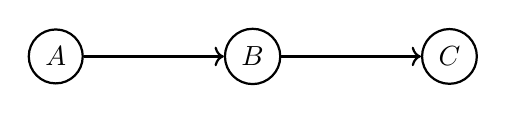
\begin{tikzpicture}[->, node distance=2.5cm, thick, main/.style = {draw, circle}]
        % Nodes
        \node[main] (A) {$A$};
        \node[main] (B) [right of=A] {$B$};
        \node[main] (C) [right of=B] {$C$};
        % Edges
        \draw (A) -- (B);
        \draw (B) -- (C);
     \end{tikzpicture}
     \end{center}
		\end{tcolorbox}
\end{frame}

\begin{frame}{Transitivity of reachability in static graphs}
  \begin{center}
    \large
    Is reachability in a temporal graph transitive?
  \end{center}
\end{frame}

\begin{frame}{Time matters!}
  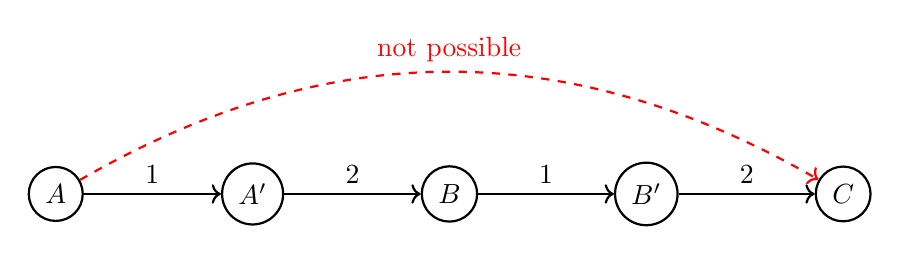
\begin{tikzpicture}[->, node distance=2.5cm, thick, main/.style = {draw, circle}]
    % Nodes
    \node[main] (A) {$A$};
    \node[main] (A_prime) [right of=A] {$A'$};
    \node[main] (B) [right of=A_prime] {$B$};
    \node[main] (B_prime) [right of=B] {$B'$};
    \node[main] (C) [right of=B_prime] {$C$};

    % Edges with time labels
    \draw (A) -- (A_prime) node[midway, above] {1};
    \draw (A_prime) -- (B) node[midway, above] {2};
    \draw (B) -- (B_prime) node[midway, above] {1};
    \draw (B_prime) -- (C) node[midway, above] {2};

    % Crossed-out edge to show non-reachability
    \draw[red, dashed] (A) edge[bend left] node[midway, above] {not possible} (C);
  \end{tikzpicture} \\[5ex]
  $\Longrightarrow$ Deep implications for complexity of temporal graphs
\end{frame}

\begin{frame}{Notation \#2}
\begin{itemize}
	\item A temporal graph $D$ is an ordered set of disjoint sets $(V, A)$
	\item $A \subseteq V^2 \times \mathbb{N}$ - 'time edges'
	\item $A(t) = \{e | (e, t) \in A\}$ - set of edges at time $t$
	\item $D(t) = (V, A(t))$ - snapshot of graph D at time $t$
\end{itemize}
\end{frame}

\begin{frame}{Static expansion of a temporal graph}
	\begin{center}
		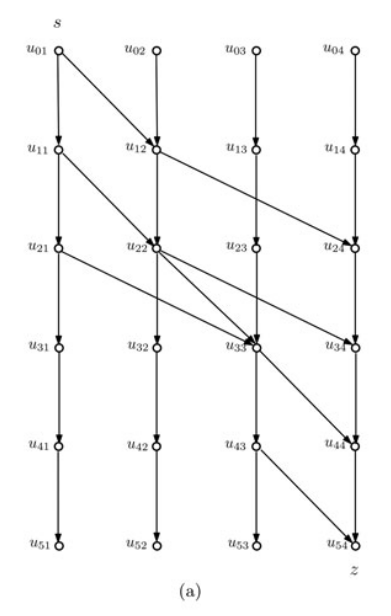
\includegraphics[height=0.8\textheight]{media/static_expansion_of_graphs.png}
	\end{center}
	\cite[page 318]{Michail2015}
\end{frame}

\begin{frame}{Static expansion of a temporal graph}
	\begin{tcolorbox}[title=Definition: static expansion of a graph]
		The static expansion of a temporal graph $D = (V, A)$ with $V = \{ u_1, u_2, ..., u_n \}$ is a DAG $H = (S, E)$ with:
		$$ S = \{ u_{ij} | \lambda_{min} - 1 \leq i \leq \lambda_{max}, 1 \leq j \leq n \} $$
		and
		$$ E = \{ (u_{(i - 1)j}, u_{ij'}) | \lambda_{min} \leq i \leq \lambda_{max} \land $$
		$$ 1 \leq j, j' \leq n \land (j = j' \lor (u_j, u_{j'}) \in A(i))) \} $$
	\end{tcolorbox}
\end{frame}

\begin{frame}{Exercise: Static expansion of a temporal graph}
  \large
  \centering
  Turn the Potsdam-Map temporal graph into its static expansion using the template given on the handout (we leave out M(edienstadt Babelsberg) for simplicity sake here) !\\
  \hfill \tiny $\approx$ 3 min
\end{frame}
\begin{frame}{Solution: Static expansion of a temporal graph}
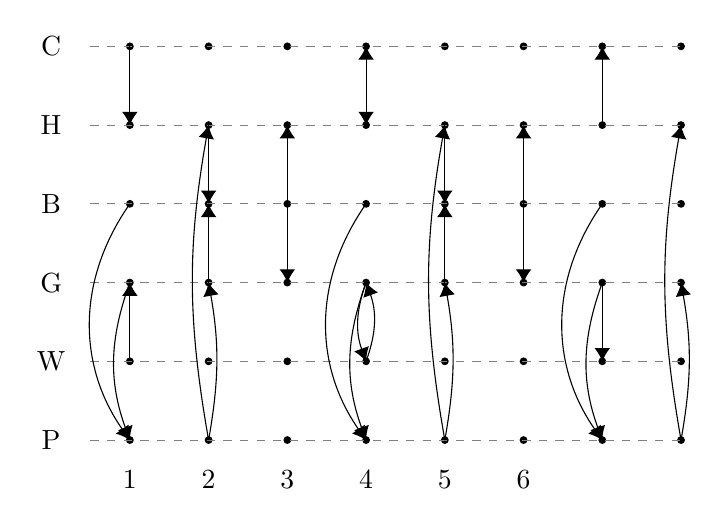
\begin{tikzpicture}
\tikzset{every arrow/.append style={arrowhead=1cm}} % Adjust scale as needed
% Define grid size
\def\rows{6} % number of rows
\def\cols{8} % number of columns

% Create nodes in a grid as small points
\foreach \i in {1, ..., \rows} {
    \foreach \j in {1, ..., \cols} {
        \node[fill=black, circle, inner sep=1pt] at (\j, -\i) {}; % small points
    }
    \draw[dashed, gray] (0.5, -\i) -- (\cols, -\i); % horizontal grid lines
    \node at(\i, -\rows - 0.5) {\i}; % row numbers
}
\node (labelC) at (0, -1) {C};
\node (labelH) at (0, -2) {H};
\node (labelB) at (0, -3) {B};
\node (labelG) at (0, -4) {G};
\node (labelW) at (0, -5) {W};
\node (labelP) at (0, -6) {P};

% C -> H
\draw[-{Latex[width=2mm]}] (1, -1) -- (1, -2);
\draw[-{Latex[width=2mm]}, bend right=20] (4, -1) -- (4, -2);
% H -> B
\draw[-{Latex[width=2mm]}] (2, -2) -- (2, -3);
\draw[-{Latex[width=2mm]}] (5, -2) -- (5, -3);
% B -> G
\draw[-{Latex[width=2mm]}] (3, -3) -- (3, -4);
\draw[-{Latex[width=2mm]}] (6, -3) -- (6, -4);
% G -> W
\draw[-{Latex[width=2mm]}, bend right=20] (4, -4) to (4, -5);
\draw[-{Latex[width=2mm]}] (7, -4) -- (7, -5);
% W -> G
\draw[-{Latex[width=2mm]}] (1, -5) to (1, -4);
\draw[-{Latex[width=2mm]}, bend right=20] (4, -5) to (4, -4);
% G -> B
\draw[-{Latex[width=2mm]}] (2, -4) to (2, -3);
\draw[-{Latex[width=2mm]}] (5, -4) to (5, -3);
% B -> H
\draw[-{Latex[width=2mm]}] (3, -3) to (3, -2);
\draw[-{Latex[width=2mm]}] (6, -3) to (6, -2);
% H -> C
\draw[-{Latex[width=2mm]}] (4, -2) to (4, -1);
\draw[-{Latex[width=2mm]}] (7, -2) to (7, -1);
% P -> B
\draw[-{Latex[width=2mm]}, bend left=10] (2, -6) to (2, -2);
\draw[-{Latex[width=2mm]}, bend left=10] (5, -6) to (5, -2);
\draw[-{Latex[width=2mm]}, bend left=10] (8, -6) to (8, -2);
% P -> G
\draw[-{Latex[width=2mm]}, bend right=10] (2, -6) to (2, -4);
\draw[-{Latex[width=2mm]}, bend right=10] (5, -6) to (5, -4);
\draw[-{Latex[width=2mm]}, bend right=10] (8, -6) to (8, -4);
% G -> P
\draw[-{Latex[width=2mm]}, bend right=20] (1, -4) to (1, -6);
\draw[-{Latex[width=2mm]}, bend right=20] (4, -4) to (4, -6);
\draw[-{Latex[width=2mm]}, bend right=20] (7, -4) to (7, -6);

% B -{Latex[width=2mm]} P
\draw[-{Latex[width=2mm]}, bend right=35] (1, -3) to (1, -6);
\draw[-{Latex[width=2mm]}, bend right=35] (4, -3) to (4, -6);
\draw[-{Latex[width=2mm]}, bend right=35] (7, -3) to (7, -6);
\end{tikzpicture}
\end{frame}



\begin{frame}{Repetition - walks and paths in static graphs}
  \begin{itemize}
    \visible<2->{
      \item A \textbf{\textit{walk}} is a finite or infinite sequence of edges which joins a sequence of vertices.
    }
    \visible<3->{
      \item A \textbf{\textit{path}} is a walk where all vertices are distinct.
    }
  \end{itemize}
\end{frame}


\begin{frame}{Journeys}
	\begin{tcolorbox}[title=Definition: temporal/time respecting walk]
		A \textbf{temporal} or \textbf{time-respecting walk} $W$ of a temporal graph $D = (V, A)$ is an alternating sequence of of nodes and times $(u_1 , t_1 , u_2 , t_2 , ... , u_{k-1} , t_{k-1} , u_k )$
		where 
		\begin{itemize}
			\item $\forall 1 \leq i \leq k - 1: ((u_i , u_{i+1} ), t_i ) \in A$ and
			\item $1 \leq i \leq k - 2: t_i < t_{i + 1}$
		\end{itemize}
	\end{tcolorbox}
	\begin{itemize}
		\item $t_1$ - departure time
		\item $t_{k - 1}$ arrival time
		\item $t_{k - 1} - t_1 + 1$ - duration/temporal length
	\end{itemize}
\end{frame}

\begin{frame}{Journeys}
	\begin{tcolorbox}[title=Definition: Journey]
		A \textbf{journey} is a is a temporal walk with pairwise distinct nodes \^{=} a journey of D is a path of the underlying static graph of D that uses
strictly increasing edge-labels.
	\end{tcolorbox}

	\visible<2->{
    \begin{tcolorbox}[title=Definition: Foremost Journey]
      A u-v journey J is called foremost from time $t \in \mathbb{N}$ if it departs after time t and its arrival time is minimized.
    \end{tcolorbox}
  }
\end{frame}

\begin{frame}{Exercise: Journeys}
  \large \centering
  What is the foremost journey from C to P in the Potsdam-Map temporal graph from time $2$?\\
\end{frame}
\againframe<1>{potsdam_city_graph}

\begin{frame}{Journeys}
	\begin{tcolorbox}[title=Definition: Temporal distance]
    The \textbf{temporal distance} from a node $u$ to at time $t$ to a node $v$ is defined as the duration of a foremost journey from $u$ to $v$ that departs at time $t$.
	\end{tcolorbox}
	\visible<2->{
	  \begin{tcolorbox}[title=Definition: Temporal diameter $d$]
     The minimum integer $d$ such that there exists a foremost journey from every node $(u, t) \in V \times \{ 0, 1, ..., \alpha - d \}$  to every node $v \in V$ with duration at most $d$.
  	\end{tcolorbox}
  }
\end{frame}

\begin{frame}{Exercise: Journeys}
  \large \centering
  Find the temporal diameter of the Potsdam-Map temporal graph.\\
\end{frame}
\againframe<1>{potsdam_city_graph}


\begin{frame}[label=foremost_journey_problem_formulation]{Computing foremost journeys - Problem formulation}
  \begin{center}
    Given a source node $s \in V$ and a start time $t_{start}$ compute the foremost $s-w$ journey for all $w \in V \text{\textbackslash{}} \{ s \}$. \\[2ex]
    Brainstorm ideas for an algorithm to solve this problem with a partner.
  \end{center}
\end{frame}

\begin{frame}{Sidenote - offline vs. online algorithms}
  \begin{minipage}{0.45\textwidth}
    \underline{offline algorithms}
    \begin{quote}
      takes whole temporal graph $D$ as input\\
    \end{quote}
    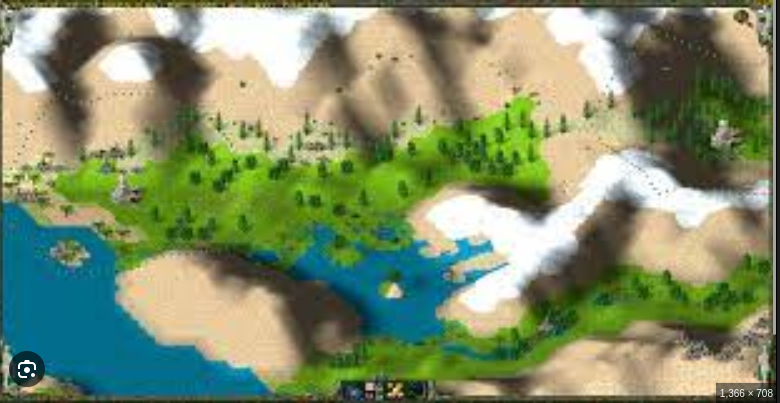
\includegraphics[width=\linewidth]{media/offline_algorithm.png}
  \end{minipage} \hfill 
  \begin{minipage}{0.45\textwidth}
    \underline{online algorithms}
    \begin{quote}
    temporal graph is revealed to algorithm over time
    \end{quote}
    
\includegraphics[width=\linewidth]{media/online_algo.png}
  \end{minipage}
  \sourcefootnote{https://encrypted-tbn0.gstatic.com/images?q=tbn:ANd9GcQbpwyZnBM48yDEHLT9Sww1J8AJrgs4lj-VLi2EkxpIoKMeI6-stF-R9uAsLl5K4gXFBts&usqp=CAU}

\end{frame}
\againframe{foremost_journey_problem_formulation}

\begin{frame}{Computing foremost journeys - Algorithm}
\begin{algorithm}[H]
\caption{Computing earliest-arrival time}
\begin{algorithmic}[1]
\footnotesize
\Require A temporal graph $G = (V, E)$ in its edge stream representation, source vertex $x$, time interval $[t_\alpha, t_\omega]$
\Ensure The earliest-arrival time from $x$ to every vertex $v \in V$ within $[t_\alpha, t_\omega]$

\State Initialize $t[x] = t_\alpha$, and $t[v] = \infty$ for all $v \in V \setminus \{x\}$
\ForAll{incoming edge $e = (u, v, t)$ in the edge stream}
    \If{$t + 1 \leq t_\omega$ and $t \geq t[u]$}
        \If{$t + 1 < t[v]$}
            \State $t[v] \gets t + 1$
        \EndIf
    \ElsIf{$t \geq t_\omega$}
        \State \textbf{break} \Comment{Go to Line 11}
    \EndIf
\EndFor
\State \Return $t[v]$ for each $v \in V$
\end{algorithmic}
\end{algorithm}
\cite{PathProblems}
\end{frame}

\begin{frame}{Computing foremost journeys - Proof of correctness}

  \begin{quote}
    Let $\mathbb{P}$ be the set of earliest-arrival paths from $x$ to a vertex $v_k$ within the time interval $[t_\alpha, t_\omega ]$. If $\mathbb{P} \not = \emptyset$ then there exists $P = (x, v_1, v_2, ..., v_k) \in \mathbb{P}$ such that every prefix-subpath, $P_i = (x, v_1, v_2, ..., v_i)$, is an earliest-arrival path from $x$ to $v_i$ within $[t_\alpha, t_\omega ]$, for $1 \leq i \leq k$.
  \end{quote} \\[3ex]
  \visible<2->{
    \begin{quote}
      For any vertex $v \in V$, if the earliest-arrival path from $x$ to $v$ within the time interval $[t_\alpha, t_\omega ]$ exists, then $t[v]$ returned by the Algorithm is the corresponding earliest-arrival time; otherwise, $t[v] = \infty$.
    \end{quote}
  }

\end{frame}

\begin{frame}{Other metrics to optimize}
  \begin{itemize}
    \item latest departure time
    \item fastest path
    \item shortest path
    \item \dots
  \end{itemize}
\end{frame}

\begin{frame}{Reachability}
	\begin{tcolorbox}[title=Definition: Reachability]
    A vertex $v$ is \textbf{reachable} from a vertex $u$ at time $t$ if there exists a foremost journey from $u$ to $v$ that departs at time $t$.
	\end{tcolorbox}
\end{frame}



\begin{frame}{The government has been lying to us}
	\begin{figure}
		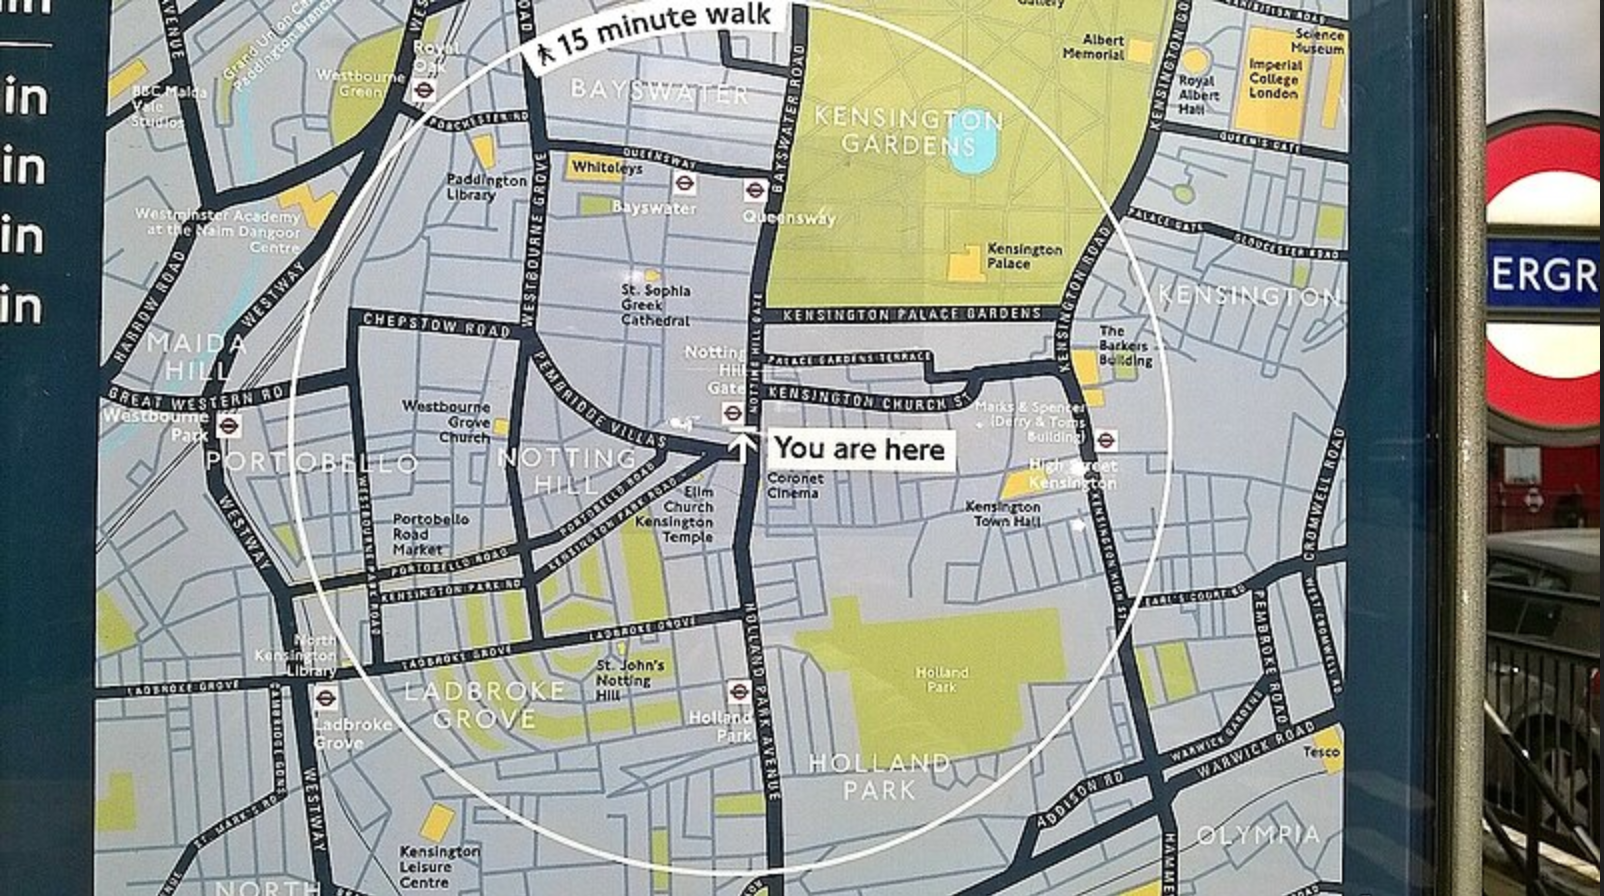
\includegraphics[width=0.9\linewidth]{media/image_1737738340.png}
		\caption{You-are-here-maps are wrong!}
	\end{figure}
	\sourcefootnote{https://commons.wikimedia.org/wiki/File:Notting_Hill_Royal_Borough_Of_K\%26C_Council_Map_Outlining_the_Official_Area_of_Notting_Hill_and_the_Surrounding_Areas_2018.jpg}
\end{frame}

\begin{frame}{15 min walk}
	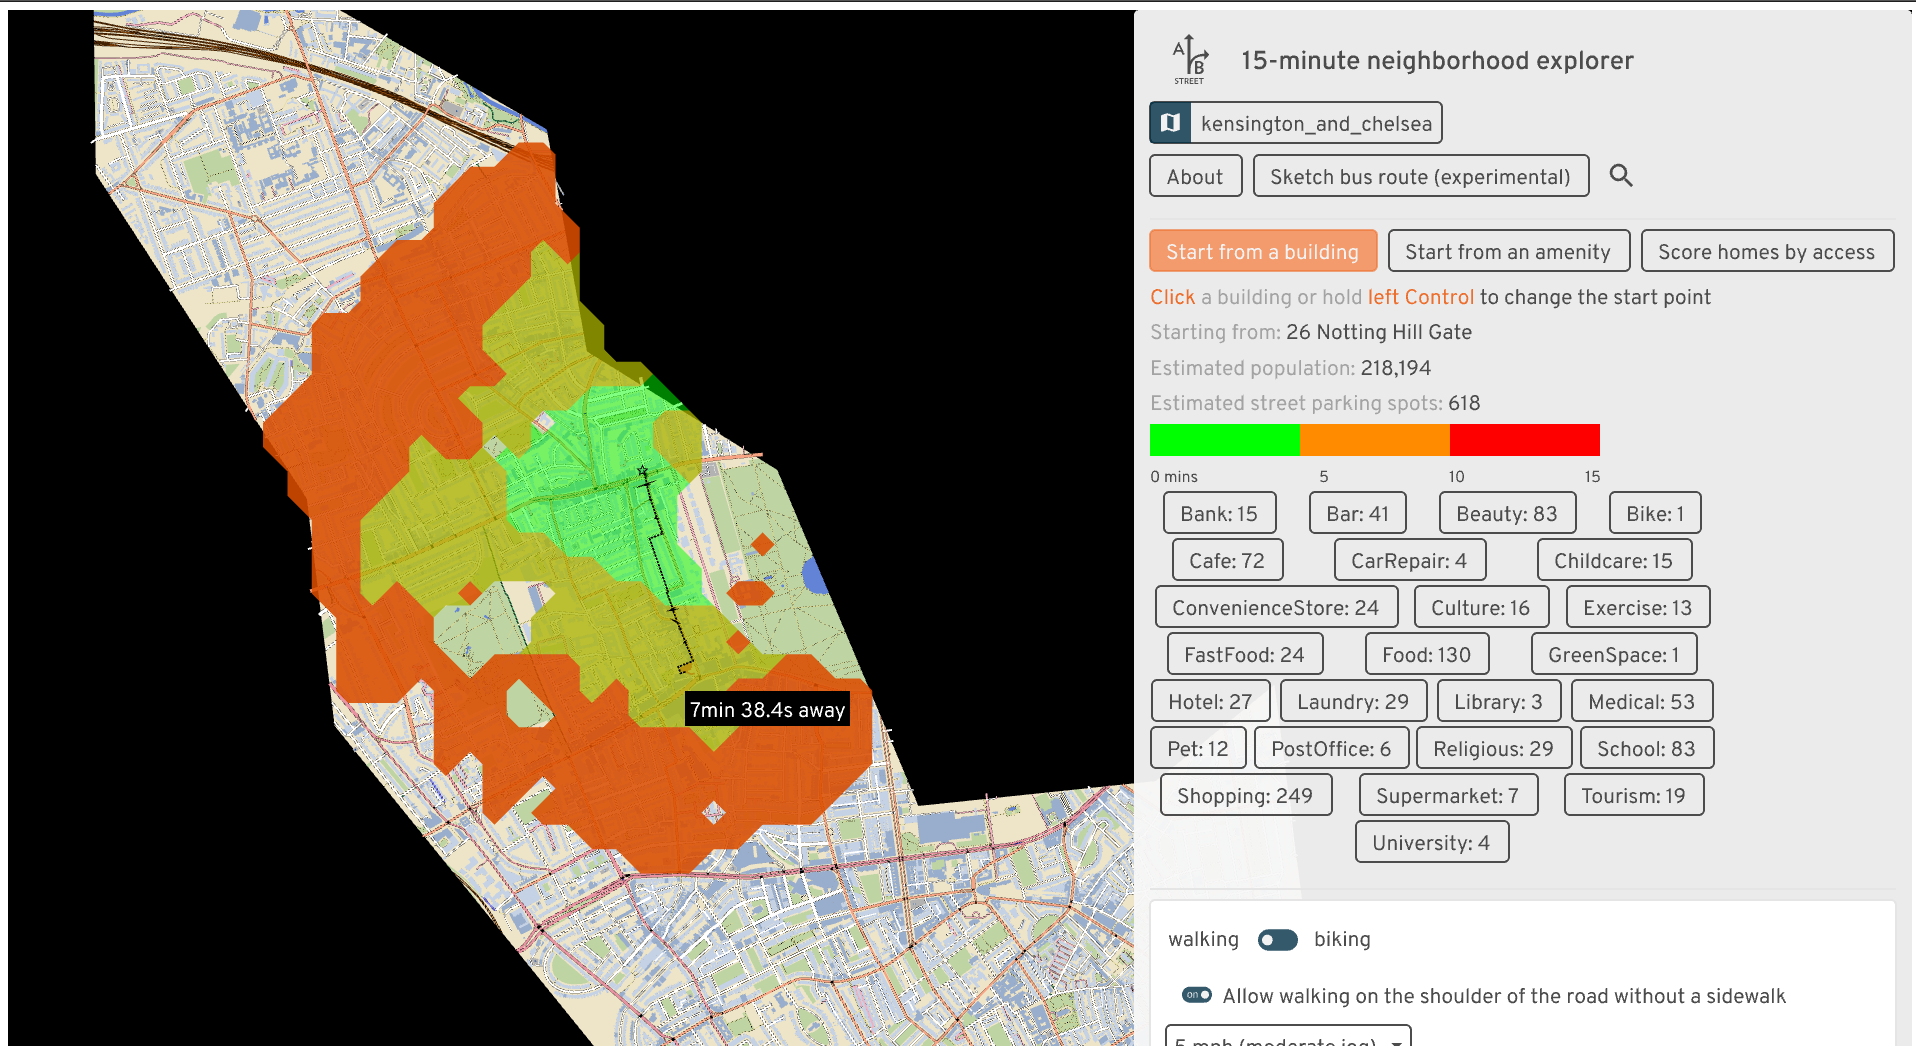
\includegraphics[width=\linewidth]{media/15-min-walk.png}
	\sourcefootnote{https://play.abstreet.org/0.3.49/fifteen_min.html}
\end{frame}


\section{Temporal graphs for modeling dissemination processes}
\begin{frame}
  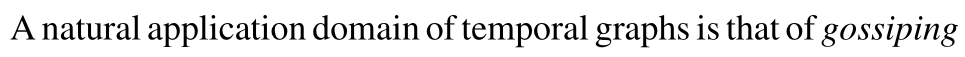
\includegraphics[width=\linewidth]{media/gossip.png} \texttildelow{} \cite{Michail2015}
\end{frame}

\begin{frame}{What are dissemination processes?}
  \centering
  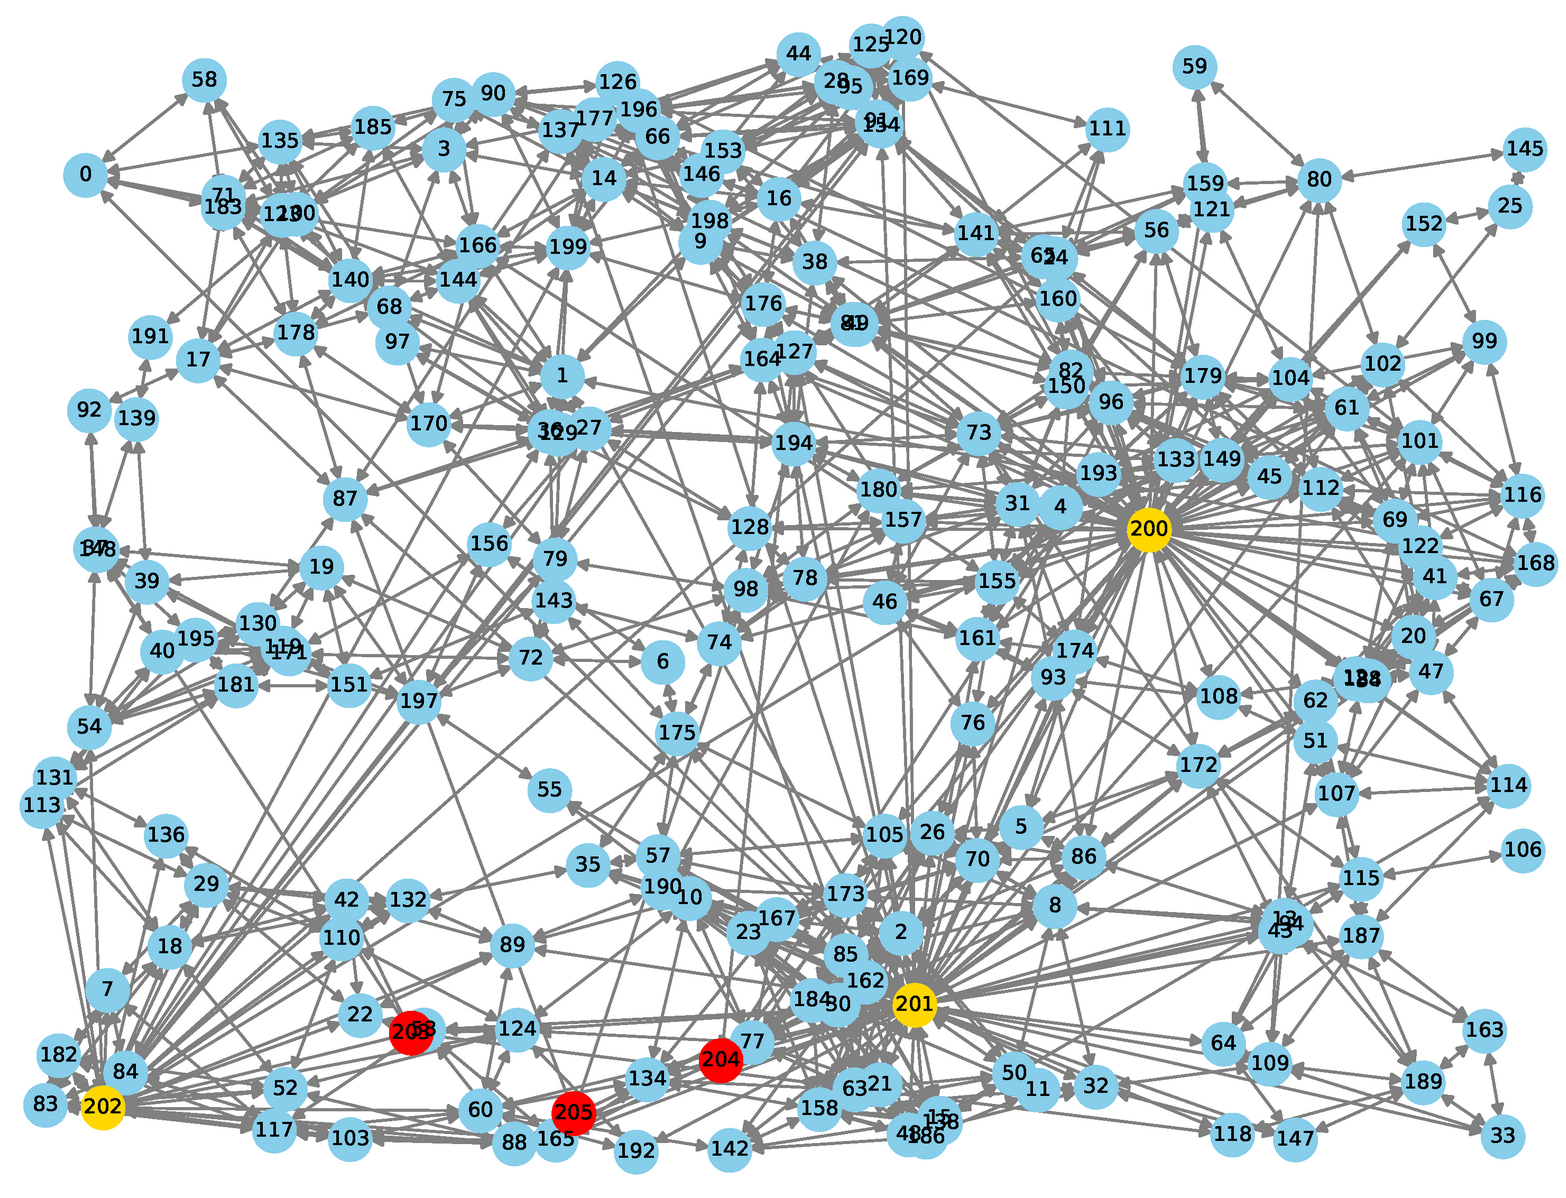
\includegraphics[width=0.9\linewidth]{media/dissemination_process_graph.png}
  \cite{fakeNews}
\end{frame}
\begin{frame}{What are dissemination processes?}
  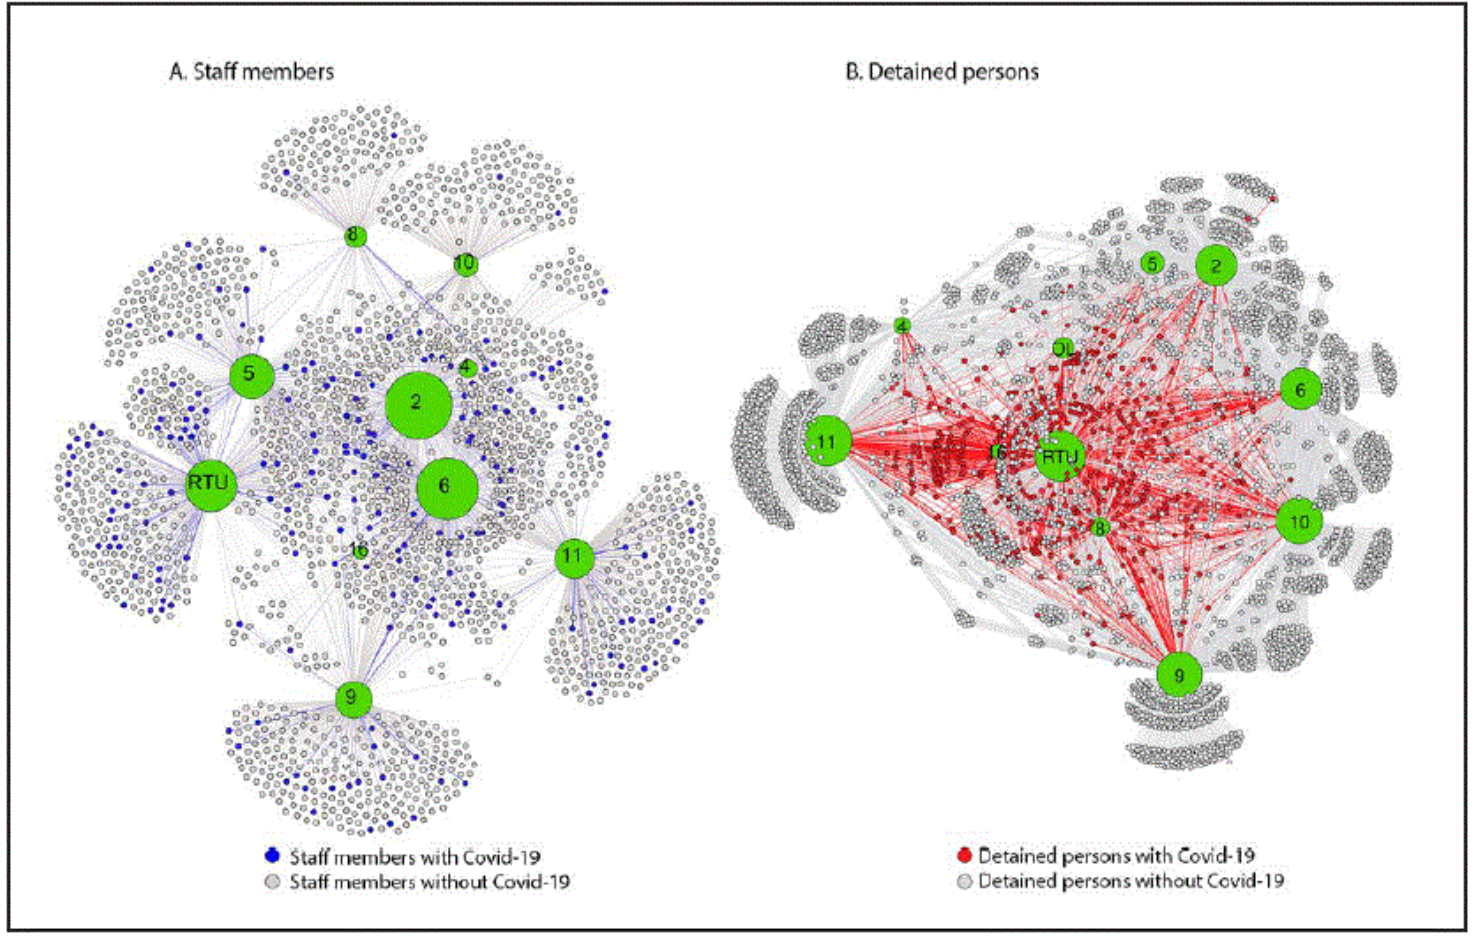
\includegraphics[width=\linewidth]{media/largeNetwork.png}
  \sourcefootnote{https://www.cdc.gov/mmwr/volumes/69/wr/figures/mm6944a3-F1.gif?_=06726}
\end{frame}
\begin{frame}{Vaccination Problem}
    \textbf{Definition:}
    The vaccination problem involves optimizing the allocation and timing of vaccines to control the spread of infectious diseases.\\
    \vspace{0.3cm} 
    \textbf{Key Questions:}
    \begin{itemize}
        \item Who should be vaccinated first?
        \item How can we minimize the spread of the disease?
        \item What role does timing play in vaccination strategies?
    \end{itemize}
    \visible<2->{
      \begin{tcolorbox}[title=Herd immunity]
        \textbf{\textit{Herd immunity}} occurs when a large enough fraction $f$ of a community is immune to a disease, thus limiting its ability to spread.
      \end{tcolorbox}
    }
    \visible<3->{
      $\Rightarrow$ lower $f$ by vaccinating people in risk
    }
\end{frame}

\begin{frame}[<+->]{Vaccination Problem - technical problem statement }
  \centering
  \begin{minipage}{0.6\textwidth}
    \large How can we \underline{optimally} chooose a fraction $f$ of a population to vaccinate using only \underline{local information}?
  \end{minipage}
\end{frame}

\begin{frame}{Vaccination Problem on static graphs}
  \begin{tcolorbox}[title=Neighbourhood Vacination protocol]
      choose a person at random among all persons that have been involved in at least one contact at time t*, ask her to name someone she met, vaccinate this other person, and repeat until a desired fraction of the vertices are vaccinated
  \end{tcolorbox}

  \begin{center}
    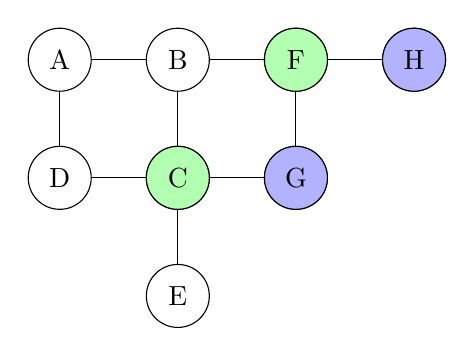
\begin{tikzpicture}[node distance=1.5cm, every node/.style={draw, circle, minimum size=0.8cm}]
        % Nodes
        \node (A) {A}; % High-risk node
        \node (B) [right of=A] {B};
        \node (C) [below of=B] {C}; % High-risk node
        \visible<3->{\node[fill=green!30] (C) [below of=B] {C};}; % High-risk node
        \node (D) [below of=A] {D};
        \node (E) [below of=C] {E};
        \node (F) [right of=B] {F};
        \visible<5, 6> {\node[fill=green!30] (F) [right of=B] {F};};
        \node (G) [below of=F] {G};
        \visible<2, 3> {\node[fill=blue!30] (G) [below of=F] {G};};
        \node (H) [right of=F] {H};
        \visible<4, 5>{\node[fill=blue!30] (I) [right of=F] {H};};

        % Edges
        \path (A) edge (B);
        \path (A) edge (D);
        \path (B) edge (C);
        \path (B) edge (F);
        \path (C) edge (D);
        \path (C) edge (E);
        \path (C) edge (G);
        \path (F) edge (G);
        \path (F) edge (H);
   \end{tikzpicture}
  \end{center}
\end{frame}

\begin{frame}{Exercise}
  \centering \large
  Discuss reasons why this strategy is so effective for eliminating the spread of a disease with a partner. \\
  \hfill \tiny 3 min
\end{frame}
\begin{frame}{Exercise}
  \begin{itemize}
    \item probability $p$ that node $a$ is infected is roughly proportional to $deg(a)$
    \item number of infected nodes is roughly proportional to $deg(a)$
    \item[$\rightarrow$] 'risk' is roughly proportional to $deg^2(a)$
  \end{itemize}
\end{frame}

\begin{frame}{Modelling dissemination processes}
  \begin{itemize}
    \item Nodes represent individuals/groups/organizations
    \item Edges represent interactions
    \item Time labels represent the time of interaction
  \end{itemize}
  \visible<2->{
  \begin{center}
    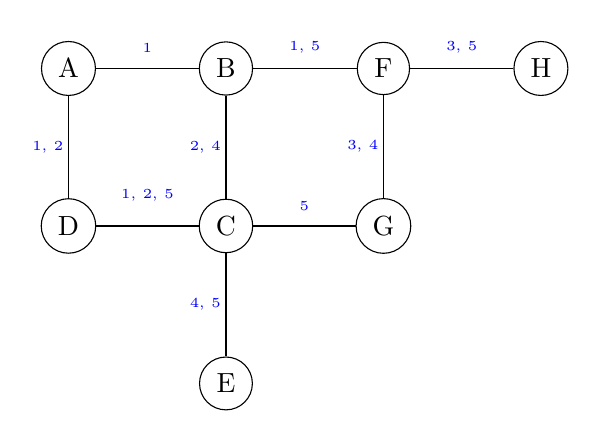
\begin{tikzpicture}[node distance=2cm, every node/.style={draw, circle, minimum size=0.5cm}]
        % Nodes
        \node (A) {A}; % High-risk node
        \node (B) [right of=A] {B};
        \node (C) [below of=B] {C}; % High-risk node
        \node (D) [below of=A] {D};
        \node (E) [below of=C] {E};
        \node (F) [right of=B] {F};
        \node (G) [below of=F] {G};
        \node (H) [right of=F] {H};

        % Edges
        \path (A) edge node[above, draw=none, font=\tiny, text=blue, inner sep=1pt] {1} (B);
        \path (A) edge node[left, draw=none, font=\tiny, text=blue, inner sep=1pt] {1, 2} (D);
        \path (B) edge node[left, draw=none, font=\tiny, text=blue, inner sep=1pt] {2, 4} (C);
        \path (B) edge node[above, draw=none, font=\tiny, text=blue, inner sep=1pt] {1, 5} (F);
        \path (C) edge node[above, draw=none, font=\tiny, text=blue, inner sep=1pt] {1, 2, 5} (D);
        \path (C) edge node[left, draw=none, font=\tiny, text=blue, inner sep=1pt] {4, 5} (E);
        \path (C) edge node[above, draw=none, font=\tiny, text=blue, inner sep=1pt] {5} (G);
        \path (F) edge node[left, draw=none, font=\tiny, text=blue, inner sep=1pt] {3, 4} (G);
        \path (F) edge node[above, draw=none, font=\tiny, text=blue, inner sep=1pt] {3, 5} (H);
   \end{tikzpicture}
  \end{center}
  }
\end{frame}

\begin{frame}{The infection process}
  \centering
  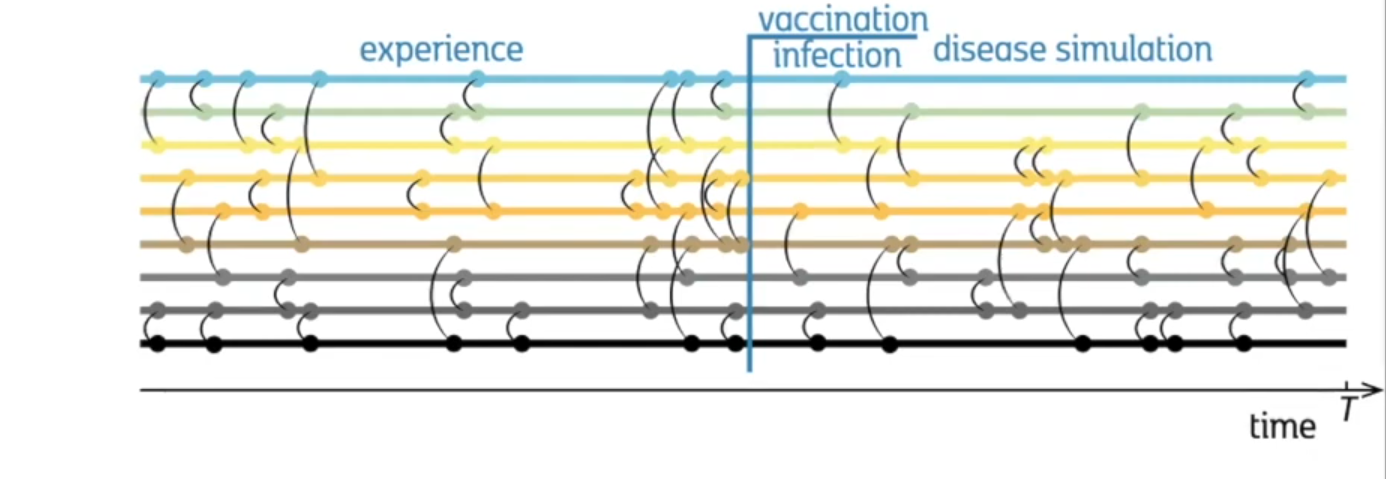
\includegraphics[width=0.7\linewidth]{media/infection_process_a.png} 

  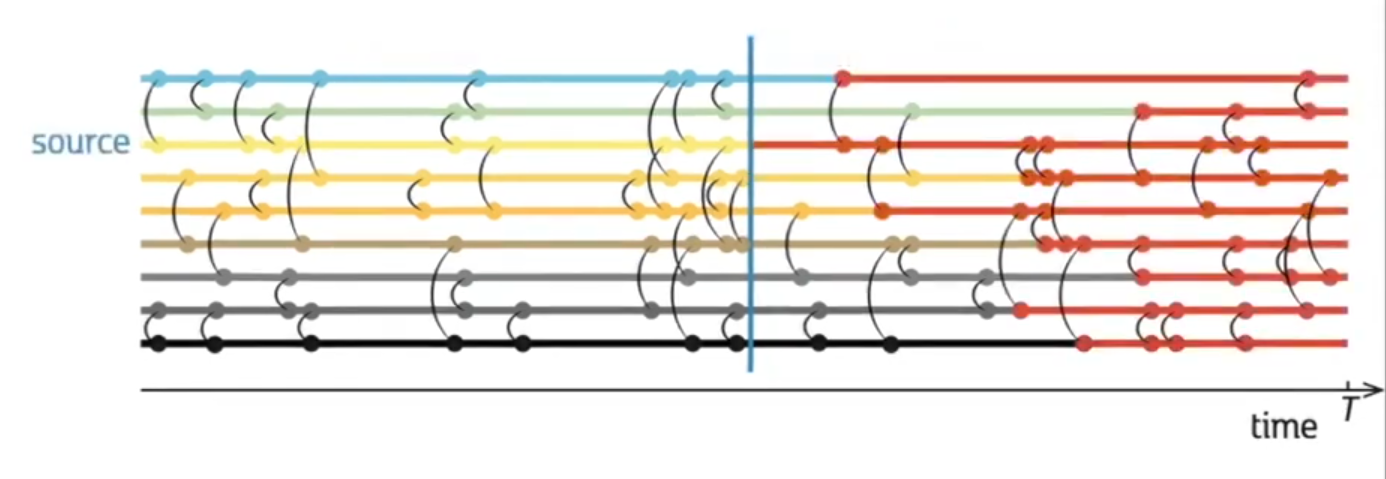
\includegraphics[width=0.7\linewidth]{media/infection_process_b.png} \\
  \cite{Lee_2012}
\end{frame}

\begin{frame}{Protocols for vaccination in temporal graphs}
  \centering 
  \begin{minipage}{0.8\textwidth}
  \large
  Brainstorm protocols that could be used to vaccinate individuals in a temporal graph. \\
  Use the neighbourhood vaccination protocol from static graphs as inspiration. \\
  \visible<2>{
    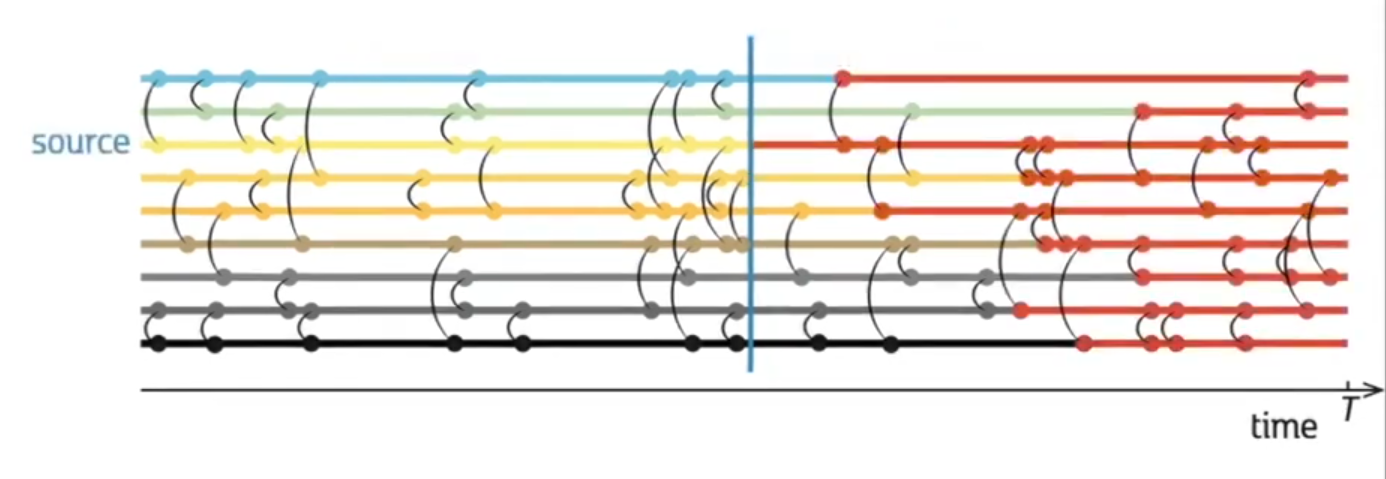
\includegraphics[width=\linewidth]{media/infection_process_b.png} \\
  }
  \small
  \hfill 4 min
  \end{minipage}
\end{frame}
\begin{frame}{Protocols for vaccination in temporal graphs}
  \begin{minipage}{0.45\textwidth}
    \textbf{\textit{Recent protocol}}  \\
    \italic{iteratively ask a random individual $I$ to name the most recent contact and vaccinated this person}
  \end{minipage}
  \hfill 
  \begin{minipage}{0.45\textwidth}
    \textbf{\textit{Weight protocol}} \\
    \italic{iteratively asked a random individual $I$ to name its most frequent contact since some time $t$ in the past}
  \end{minipage}
  \vspace*{2cm}
  \visible<2->{
    Apply those two protocols to the given temporal graphs on your handout. Then, discuss how the performance of the protocols might scale in real-world data (e.g. contacts in hospital, on a dating website, ...). \hfill \small \textit{6min}
  }
\end{frame}

\begin{frame}{Solution}
  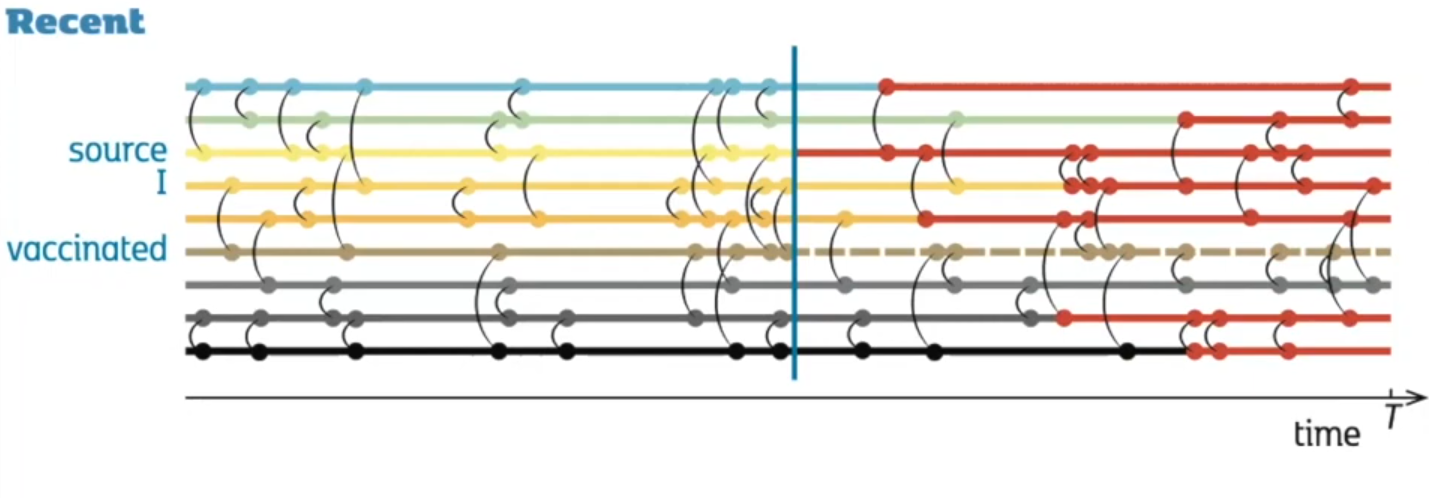
\includegraphics[width=\linewidth]{media/solution_recent.png}
  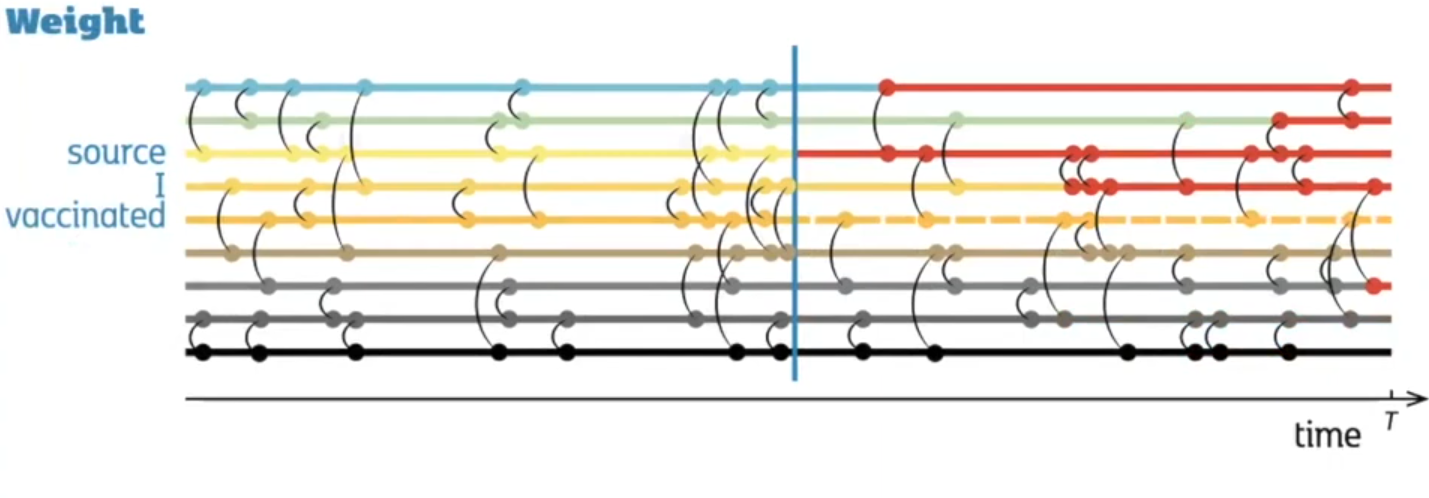
\includegraphics[width=\linewidth]{media/solution_weight.png} 
\end{frame}

\begin{frame}{Performance on bigger datasets}
  \centering
  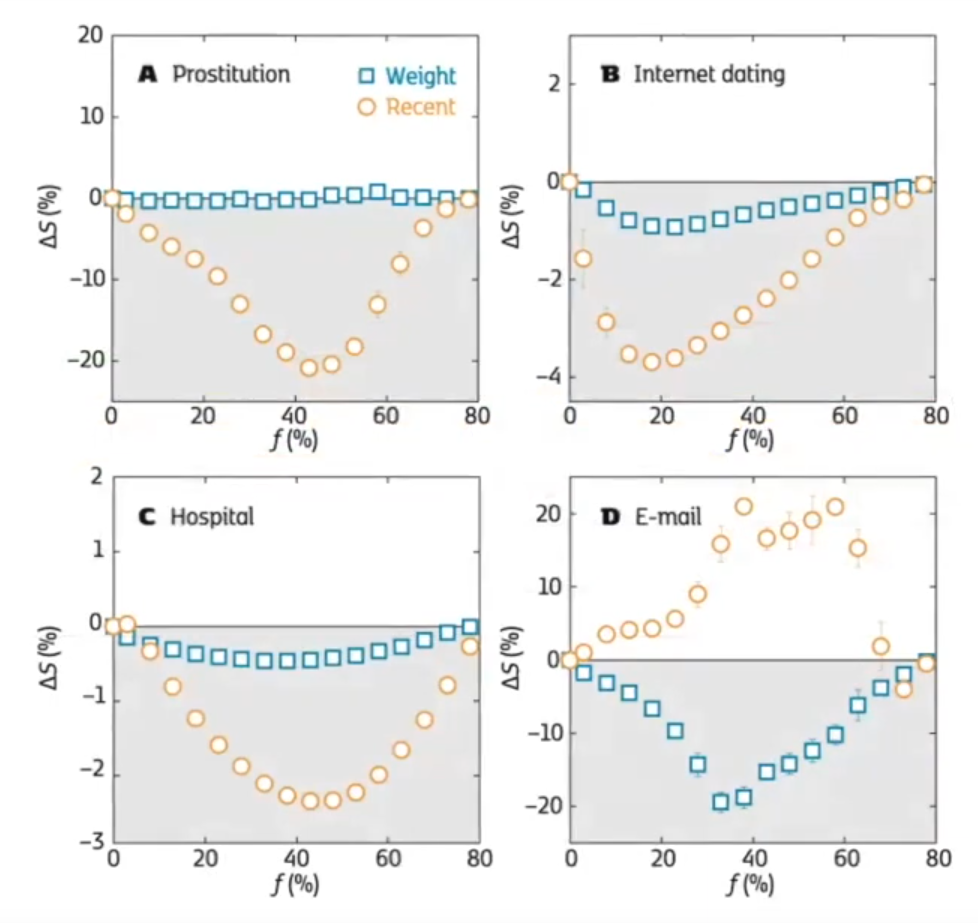
\includegraphics[width=0.6\linewidth]{media/performance_protocols.png}
  \cite{Lee_2012}
\end{frame}

\section{Teasers}
\begin{frame}{Further interesting problems on temporal graphs}
  \begin{itemize}
    \item Centrality of nodes in a temporal graph
    \item temporal graph metrics
    \item temporal connectivity
    \item Temporal Graph Neural Networks
  \end{itemize}
\end{frame}

\begin{frame}[allowframebreaks]{Sources}
  \bibliographystyle{plain} % Choose a bibliography style
  \bibliography{references} % Path to your .bib file
\end{frame}

\end{document}
